\documentclass[twoside]{book}

% Packages required by doxygen
\usepackage{calc}
\usepackage{doxygen}
\usepackage{graphicx}
\usepackage[utf8]{inputenc}
\usepackage{makeidx}
\usepackage{multicol}
\usepackage{multirow}
\usepackage{textcomp}
\usepackage[table]{xcolor}

% Font selection
\usepackage[T1]{fontenc}
\usepackage{mathptmx}
\usepackage[scaled=.90]{helvet}
\usepackage{courier}
\usepackage{amssymb}
\usepackage{sectsty}
\renewcommand{\familydefault}{\sfdefault}
\allsectionsfont{%
  \fontseries{bc}\selectfont%
  \color{darkgray}%
}
\renewcommand{\DoxyLabelFont}{%
  \fontseries{bc}\selectfont%
  \color{darkgray}%
}

% Page & text layout
\usepackage{geometry}
\geometry{%
  a4paper,%
  top=2.5cm,%
  bottom=2.5cm,%
  left=2.5cm,%
  right=2.5cm%
}
\tolerance=750
\hfuzz=15pt
\hbadness=750
\setlength{\emergencystretch}{15pt}
\setlength{\parindent}{0cm}
\setlength{\parskip}{0.2cm}
\makeatletter
\renewcommand{\paragraph}{%
  \@startsection{paragraph}{4}{0ex}{-1.0ex}{1.0ex}{%
    \normalfont\normalsize\bfseries\SS@parafont%
  }%
}
\renewcommand{\subparagraph}{%
  \@startsection{subparagraph}{5}{0ex}{-1.0ex}{1.0ex}{%
    \normalfont\normalsize\bfseries\SS@subparafont%
  }%
}
\makeatother

% Headers & footers
\usepackage{fancyhdr}
\pagestyle{fancyplain}
\fancyhead[LE]{\fancyplain{}{\bfseries\thepage}}
\fancyhead[CE]{\fancyplain{}{}}
\fancyhead[RE]{\fancyplain{}{\bfseries\leftmark}}
\fancyhead[LO]{\fancyplain{}{\bfseries\rightmark}}
\fancyhead[CO]{\fancyplain{}{}}
\fancyhead[RO]{\fancyplain{}{\bfseries\thepage}}
\fancyfoot[LE]{\fancyplain{}{}}
\fancyfoot[CE]{\fancyplain{}{}}
\fancyfoot[RE]{\fancyplain{}{\bfseries\scriptsize Generated on Fri Oct 27 2017 09\-:24\-:01 for superquadric-\/grasp-\/example by Doxygen }}
\fancyfoot[LO]{\fancyplain{}{\bfseries\scriptsize Generated on Fri Oct 27 2017 09\-:24\-:01 for superquadric-\/grasp-\/example by Doxygen }}
\fancyfoot[CO]{\fancyplain{}{}}
\fancyfoot[RO]{\fancyplain{}{}}
\renewcommand{\footrulewidth}{0.4pt}
\renewcommand{\chaptermark}[1]{%
  \markboth{#1}{}%
}
\renewcommand{\sectionmark}[1]{%
  \markright{\thesection\ #1}%
}

% Indices & bibliography
\usepackage{natbib}
\usepackage[titles]{tocloft}
\setcounter{tocdepth}{3}
\setcounter{secnumdepth}{5}
\makeindex

% Hyperlinks (required, but should be loaded last)
\usepackage{ifpdf}
\ifpdf
  \usepackage[pdftex,pagebackref=true]{hyperref}
\else
  \usepackage[ps2pdf,pagebackref=true]{hyperref}
\fi
\hypersetup{%
  colorlinks=true,%
  linkcolor=blue,%
  citecolor=blue,%
  unicode%
}

% Custom commands
\newcommand{\clearemptydoublepage}{%
  \newpage{\pagestyle{empty}\cleardoublepage}%
}


%===== C O N T E N T S =====

\begin{document}

% Titlepage & ToC
\pagenumbering{roman}
\begin{titlepage}
\vspace*{7cm}
\begin{center}%
{\Large superquadric-\/grasp-\/example }\\
\vspace*{1cm}
{\large Generated by Doxygen 1.8.6}\\
\vspace*{0.5cm}
{\small Fri Oct 27 2017 09:24:01}\\
\end{center}
\end{titlepage}
\clearemptydoublepage
\tableofcontents
\clearemptydoublepage
\pagenumbering{arabic}

%--- Begin generated contents ---
\chapter{Module Index}
\section{Modules}
Here is a list of all modules\-:\begin{DoxyCompactList}
\item \contentsline{section}{experiment-\/1}{\pageref{group__experiment-1}}{}
\end{DoxyCompactList}

\chapter{Hierarchical Index}
\section{Class Hierarchy}
This inheritance list is sorted roughly, but not completely, alphabetically\-:\begin{DoxyCompactList}
\item \contentsline{section}{experiment\-One\-\_\-\-I\-D\-L}{\pageref{classexperimentOne__IDL}}{}
\begin{DoxyCompactList}
\item \contentsline{section}{Experiment\-One}{\pageref{classExperimentOne}}{}
\end{DoxyCompactList}
\end{DoxyCompactList}

\chapter{Data Structure Index}
\section{Data Structures}
Here are the data structures with brief descriptions\-:\begin{DoxyCompactList}
\item\contentsline{section}{\hyperlink{classExperimentOne}{Experiment\-One} \\*Wrapper for the superquadric modeling and grasping frameworks }{\pageref{classExperimentOne}}{}
\item\contentsline{section}{\hyperlink{classexperimentOne__IDL}{experiment\-One\-\_\-\-I\-D\-L} \\*Experiment\-One\-\_\-\-I\-D\-L I\-D\-L Interface to \hyperlink{group__experiment-1}{experiment-\/1} services }{\pageref{classexperimentOne__IDL}}{}
\end{DoxyCompactList}

\chapter{Module Documentation}
\section{experiment-\/1}
\label{group__experiment-1}\index{experiment-\/1@{experiment-\/1}}


An example on how to run the superquadric modeling and grasping demo.  


An example on how to run the superquadric modeling and grasping demo. Version\-:1.\-0 \begin{DoxyAuthor}{Author}
Giulia Vezzani \href{mailto:giulia.vezzani@iit.it}{\tt giulia.\-vezzani@iit.\-it} \par
 
\end{DoxyAuthor}
\begin{DoxyCopyright}{Copyright}
Released under the terms of the G\-N\-U G\-P\-L v2.\-0 
\end{DoxyCopyright}
\hypertarget{group__experiment-1_intro_sec}{}\subsection{Description}\label{group__experiment-1_intro_sec}
This module provides a wrapper code for performing the superquadric modeling and grasping demo. A tutorial on how to use the module is provided here\-: \href{https://github.com/robotology/superquadric-grasp-example/tree/gh-pages/experiment-1#how-to-run-the-code}{\tt {\bfseries tutorial}}.

This page illustrates the main parameters of the module (Section {\bfseries Parameters}), the available ports and services.\hypertarget{group__experiment-1_parameters_sec}{}\subsection{Parameters}\label{group__experiment-1_parameters_sec}

\begin{DoxyItemize}
\item --from\-: Configuration file name.
\item --objname\-: The name of the object to be modeled and grasped.
\item --hand\-\_\-for\-\_\-computing\-: Select the hand for which we want to compute a grasping pose. Available values\-: right, left, both.
\item --hand\-\_\-for\-\_\-computing\-: Select the hand for which we want to use for executing the grasping. Available values\-: right, left. 
\end{DoxyItemize}\hypertarget{group__experiment-1_inputports_sec}{}\subsection{Input Ports}\label{group__experiment-1_inputports_sec}

\begin{DoxyItemize}
\item /experiment-\/1/img\-:i \mbox{[}yarp\-::sig\-::\-Image\-Of\-Pixel\-Rgb\mbox{]} \mbox{[}default carrier\-:tcp\mbox{]}\-: Receive the image from the left camera for saving the colored point cloud.
\end{DoxyItemize}\hypertarget{group__experiment-1_outputports_sec}{}\subsection{Output Ports}\label{group__experiment-1_outputports_sec}
\hypertarget{group__experiment-1_services_sec}{}\subsection{Services}\label{group__experiment-1_services_sec}

\begin{DoxyItemize}
\item /experiment-\/1/rpc \mbox{[}rpc-\/server\mbox{]}\-: service port . This service is described in \hyperlink{classexperimentOne__IDL}{experiment\-One\-\_\-\-I\-D\-L} (idl.\-thrift)
\item /experiment-\/1/blob\-:rpc \mbox{[}rpc-\/client\mbox{]}\-:

Ask for the 2\-D blob of the object.

. This service is described in yarp\-::os\-::\-Bottle ()
\item /experiment-\/1/\-O\-P\-C\-:rpc \mbox{[}rpc-\/client\mbox{]}\-:

Ask for the 2\-D bounding box of the object.

. This service is described in yarp\-::os\-::\-Bottle ()
\item /experiment-\/1/\-S\-F\-M\-:rpc \mbox{[}rpc-\/client\mbox{]}\-:

Ask for the 3\-D point cloud of the object.

. This service is described in yarp\-::os\-::\-Bottle ()
\item /experiment-\/1/superq\-:rpc \mbox{[}rpc-\/client\mbox{]}\-:

Interact with the superquadric-\/model module.

. This service is described in yarp\-::os\-::\-Bottle ()
\item /experiment-\/1/grasp\-:rpc \mbox{[}rpc-\/client\mbox{]}\-:

Interact with the superquadric-\/grasp module.

. This service is described in yarp\-::os\-::\-Bottle () 
\end{DoxyItemize}
\chapter{Data Structure Documentation}
\section{Experiment\-One Class Reference}
\label{classExperimentOne}\index{Experiment\-One@{Experiment\-One}}


The \hyperlink{classExperimentOne}{Experiment\-One} class provides a wrapper for the superquadric modeling and grasping frameworks.  


Inheritance diagram for Experiment\-One\-:\begin{figure}[H]
\begin{center}
\leavevmode
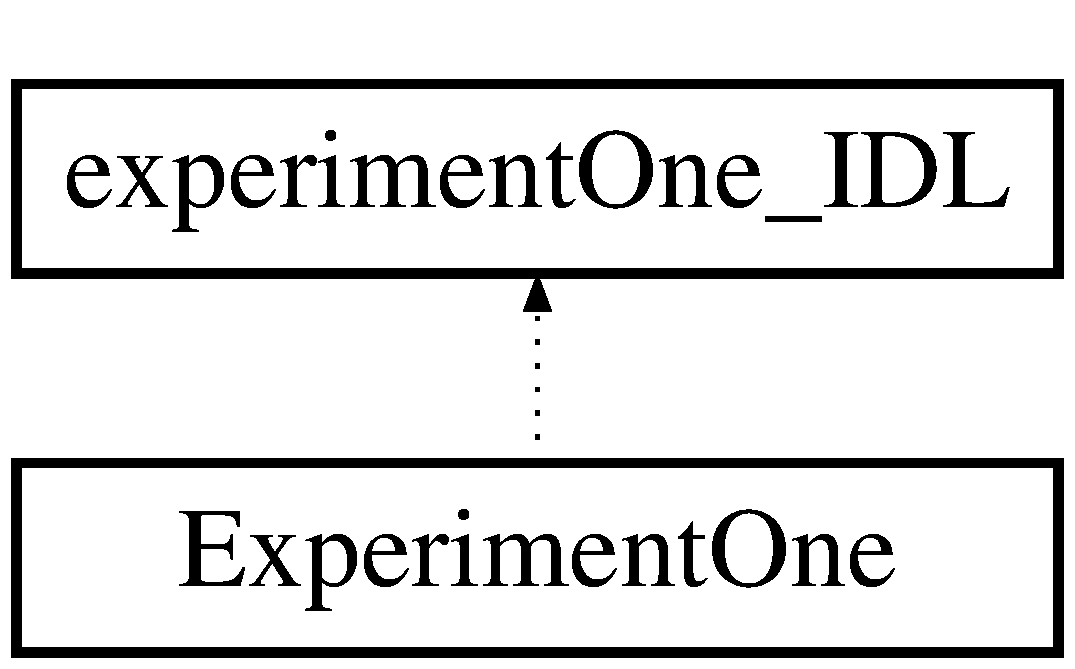
\includegraphics[height=2.000000cm]{classExperimentOne}
\end{center}
\end{figure}
\subsection*{Public Member Functions}
\begin{DoxyCompactItemize}
\item 
bool {\bfseries attach} (Rpc\-Server \&source)\label{classExperimentOne_a99a9e579f4a79b7a41c445c6a14a45f3}

\item 
Bottle \hyperlink{classExperimentOne_ad36ac49e1121169c5a38e50fa3684023}{get\-\_\-\-Blob} ()
\begin{DoxyCompactList}\small\item\em Send the current 2\-D blob. \end{DoxyCompactList}\item 
bool \hyperlink{classExperimentOne_a9f29aa4b81d957c693e4555cb4c06ccb}{set\-\_\-object\-\_\-name} (const string \&object\-\_\-name)
\begin{DoxyCompactList}\small\item\em Set the name of the object (stored by the object property collector). \end{DoxyCompactList}\item 
string \hyperlink{classExperimentOne_ac087378ef3308b52cef17a2fc9d80dfe}{get\-\_\-object\-\_\-name} ()
\begin{DoxyCompactList}\small\item\em Get the name of the object. \end{DoxyCompactList}\item 
bool \hyperlink{classExperimentOne_a9f4bc21cb93ecd4d4bdebb29ef2684cf}{set\-\_\-hand\-\_\-for\-\_\-computation} (const string \&h)
\begin{DoxyCompactList}\small\item\em Set the hand for pose computation. \end{DoxyCompactList}\item 
string \hyperlink{classExperimentOne_aef03af801993c3d869f0eedde21388dd}{get\-\_\-hand\-\_\-for\-\_\-computation} ()
\begin{DoxyCompactList}\small\item\em Get the hand for pose computation. \end{DoxyCompactList}\item 
bool \hyperlink{classExperimentOne_af9b4928dcc41cdd499f1e81bd7004ba7}{set\-\_\-hand\-\_\-for\-\_\-moving} (const string \&h)
\begin{DoxyCompactList}\small\item\em Set the hand for moving. \end{DoxyCompactList}\item 
string \hyperlink{classExperimentOne_a066ac71cee6dec9422f213b2a58f21ba}{get\-\_\-hand\-\_\-for\-\_\-moving} ()
\begin{DoxyCompactList}\small\item\em Get the hand for pose computation. \end{DoxyCompactList}\item 
string \hyperlink{classExperimentOne_a25eb29db579ef1d960c35bd2bc71ec36}{get\-\_\-automatic\-\_\-hand} ()
\begin{DoxyCompactList}\small\item\em Get if automatic selection of the hand is on or off. \end{DoxyCompactList}\item 
bool \hyperlink{classExperimentOne_a3bb4965701fe8b4062d974f0c75f5355}{set\-\_\-automatic\-\_\-hand} (const string \&entry)
\begin{DoxyCompactList}\small\item\em Set if automatic selection of the hand is on or off. \end{DoxyCompactList}\item 
bool \hyperlink{classExperimentOne_a6ce79bc38d0e6fc201db5576a2c9e265}{go\-\_\-next} ()
\begin{DoxyCompactList}\small\item\em Ask to go to the next step, following the pipeline\-: 1-\/ compute superquadric 2-\/ compute pose 3-\/ ask the robot to move. \end{DoxyCompactList}\item 
bool \hyperlink{classExperimentOne_ac01beb32e67fd6067c273ae505060139}{start\-\_\-from\-\_\-scratch} ()
\begin{DoxyCompactList}\small\item\em The pipeline is restarted and is waiting the command \char`\"{}go\-\_\-next\char`\"{} to start from step 1. \end{DoxyCompactList}\item 
bool \hyperlink{classExperimentOne_a28e92b0a8df58c9dfc77ddae39c642b5}{acquire\-\_\-superq} ()
\begin{DoxyCompactList}\small\item\em If you want just to perform step 1. \end{DoxyCompactList}\item 
bool \hyperlink{classExperimentOne_a39a4ec1aa004bcdc7a2b3cfb3804e59f}{compute\-\_\-pose} ()
\begin{DoxyCompactList}\small\item\em If you want just to perform step 2 (if step 1 has been performed). \end{DoxyCompactList}\item 
bool \hyperlink{classExperimentOne_a9a2ab97ed5ae9420e352a20b01feda90}{grasp\-\_\-object} ()
\begin{DoxyCompactList}\small\item\em If you want just to perform step 3 (if step 2 has been performed). \end{DoxyCompactList}\item 
bool \hyperlink{classExperimentOne_a967da7276e9bee19c45c8a000bf1cb01}{go\-\_\-back\-\_\-home} ()
\begin{DoxyCompactList}\small\item\em Ask the robot to stop and go back to home position with the arm that is moving. \end{DoxyCompactList}\item 
bool \hyperlink{classExperimentOne_a827996b603991113f08c928ccd7e7793}{clear\-\_\-poses} ()
\begin{DoxyCompactList}\small\item\em Clear all the computed poses. \end{DoxyCompactList}\item 
bool \hyperlink{classExperimentOne_a88d1dd39e2a145d6042bd6d2203a69eb}{set\-\_\-filtered\-\_\-superq} (const string \&entry)
\begin{DoxyCompactList}\small\item\em Set if to ask the filtered superquadric or not. \end{DoxyCompactList}\item 
string \hyperlink{classExperimentOne_a4fcbf7d582b26a64f67fc7d05f578e41}{get\-\_\-filtered\-\_\-superq} ()
\begin{DoxyCompactList}\small\item\em Get if to ask the filtered superquadric or not. \end{DoxyCompactList}\item 
bool \hyperlink{classExperimentOne_a9a0ab63f624d2ec7f36f765b3102050e}{set\-\_\-reset\-\_\-filter} (const string \&entry)
\begin{DoxyCompactList}\small\item\em Set if to reset the filtered superquadric or not. \end{DoxyCompactList}\item 
string \hyperlink{classExperimentOne_a3573bd59ace3a48477beefb75d544326}{get\-\_\-reset\-\_\-filter} ()
\begin{DoxyCompactList}\small\item\em Get if to reset the filtered superquadric or not. \end{DoxyCompactList}\item 
bool \hyperlink{classExperimentOne_a4edd34a85b30715ee7d2dda9ea277e91}{set\-\_\-object\-\_\-class} (const string \&entry)
\begin{DoxyCompactList}\small\item\em Set the current object class. \end{DoxyCompactList}\item 
string \hyperlink{classExperimentOne_a43cf934e2479fd6ef87be9048800a489}{get\-\_\-object\-\_\-class} ()
\begin{DoxyCompactList}\small\item\em Get the current object class. \end{DoxyCompactList}\item 
bool \hyperlink{classExperimentOne_af4d06d36f98664027740e2f2587411db}{getperiod} ()
\begin{DoxyCompactList}\small\item\em Set the R\-F\-Module period. \end{DoxyCompactList}\item 
bool \hyperlink{classExperimentOne_acdfcaf1bcef7810b260ee74afd6479bf}{configure} (Resource\-Finder \&rf)
\begin{DoxyCompactList}\small\item\em Configure method of the R\-F\-Module. \end{DoxyCompactList}\item 
bool \hyperlink{classExperimentOne_a6ceff4b470d8800ac941cc813270ff4b}{close} ()
\begin{DoxyCompactList}\small\item\em Close all the ports. \end{DoxyCompactList}\item 
bool \hyperlink{classExperimentOne_a77236f66f20d8f82d06c7aac1314a1bd}{update\-Module} ()
\begin{DoxyCompactList}\small\item\em Execute the state machine and the communications with external modules. \end{DoxyCompactList}\item 
void \hyperlink{classExperimentOne_ad988faee9be73dfabf529d8bf43f421d}{get\-Blob} ()\label{classExperimentOne_ad988faee9be73dfabf529d8bf43f421d}

\begin{DoxyCompactList}\small\item\em Acquire 2\-D blob of the object. \end{DoxyCompactList}\item 
void \hyperlink{classExperimentOne_ac815fad9912cd04f2f512efbb1f67571}{point\-From\-Name} ()\label{classExperimentOne_ac815fad9912cd04f2f512efbb1f67571}

\begin{DoxyCompactList}\small\item\em Get object 2\-D center from its name. \end{DoxyCompactList}\item 
deque$<$ Vector $>$ \hyperlink{classExperimentOne_a4c489f3fed0a7bac019895adb66807cb}{get3\-Dpoints} (Image\-Of$<$ Pixel\-Rgb $>$ $\ast$Img\-In)
\begin{DoxyCompactList}\small\item\em Get 3\-D points by querying S\-F\-M. \end{DoxyCompactList}\item 
bool \hyperlink{classExperimentOne_aa6abe663d8234c25e19460370cde408e}{read\-Superq} (const string \&name\-\_\-obj, Vector \&x, const int \&dimension, Resource\-Finder $\ast$rf)
\begin{DoxyCompactList}\small\item\em Read the superquadric from the configuration file, in offline mode. \end{DoxyCompactList}\item 
Property \hyperlink{classExperimentOne_a725e2b788b64d85d38e33b8d52ed5d02}{fill\-Property} (const Vector \&sol)
\begin{DoxyCompactList}\small\item\em Fill a property with the solutions inside. \end{DoxyCompactList}\item 
void \hyperlink{classExperimentOne_a0c8125d92c65d43c55c97adc32c5c576}{get\-Bottle} (Bottle \&estimated\-\_\-superq, Bottle \&cmd)\label{classExperimentOne_a0c8125d92c65d43c55c97adc32c5c576}

\begin{DoxyCompactList}\small\item\em Process bottle with the superquadric. \end{DoxyCompactList}\end{DoxyCompactItemize}
\subsection*{Private Member Functions}
\begin{DoxyCompactItemize}
\item 
virtual yarp\-::os\-::\-Bottle \hyperlink{classexperimentOne__IDL_a4e631c4039aa9e4685f7d75f778145a2}{get\-\_\-blob} ()
\begin{DoxyCompactList}\small\item\em Send the current 2\-D blob. \end{DoxyCompactList}\item 
virtual bool \hyperlink{classexperimentOne__IDL_a3ba4eae42268c1dec8c90a971ffde7af}{set\-\_\-object\-\_\-name} (const std\-::string \&entry)
\begin{DoxyCompactList}\small\item\em Set the name of the object (stored by the object property collector). \end{DoxyCompactList}\item 
virtual bool \hyperlink{classexperimentOne__IDL_acb2bfe937ed1900166744fce3a8f4cab}{set\-\_\-hand\-\_\-for\-\_\-computation} (const std\-::string \&entry)
\begin{DoxyCompactList}\small\item\em Set the hand for pose computation. \end{DoxyCompactList}\item 
virtual bool \hyperlink{classexperimentOne__IDL_a0422e6ffaef0e60e1a557a342aeb5d4a}{set\-\_\-hand\-\_\-for\-\_\-moving} (const std\-::string \&entry)
\begin{DoxyCompactList}\small\item\em Set the hand for moving. \end{DoxyCompactList}\item 
virtual bool \hyperlink{classexperimentOne__IDL_a1612f36ed85af9e6dbc595405e733977}{set\-\_\-automatic\-\_\-hand} (const std\-::string \&entry)
\begin{DoxyCompactList}\small\item\em Set if automatic selection of the hand is on or off. \end{DoxyCompactList}\item 
virtual bool \hyperlink{classexperimentOne__IDL_a36a7306993eeae5778bacac4f4154126}{set\-\_\-filtered\-\_\-superq} (const std\-::string \&entry)
\begin{DoxyCompactList}\small\item\em Set if to ask the filtered superquadric or not. \end{DoxyCompactList}\item 
virtual bool \hyperlink{classexperimentOne__IDL_a0e42d009f1d2bfbaae9906c4775dd922}{set\-\_\-reset\-\_\-filter} (const std\-::string \&entry)
\begin{DoxyCompactList}\small\item\em Set if to reset the filtered superquadric or not. \end{DoxyCompactList}\item 
virtual bool \hyperlink{classexperimentOne__IDL_a12be87d589038ab4ee9bc1adb902ac53}{set\-\_\-object\-\_\-class} (const std\-::string \&entry)
\begin{DoxyCompactList}\small\item\em Set the current object class. \end{DoxyCompactList}\item 
virtual bool {\bfseries read} (yarp\-::os\-::\-Connection\-Reader \&connection) Y\-A\-R\-P\-\_\-\-O\-V\-E\-R\-R\-I\-D\-E\label{classexperimentOne__IDL_a3e02eb2decd566b824035195358abe0d}

\item 
virtual std\-::vector$<$ std\-::string $>$ {\bfseries help} (const std\-::string \&function\-Name=\char`\"{}-\/-\/all\char`\"{})\label{classexperimentOne__IDL_a758e17bcfb1b243915cd696eccd1ce5b}

\end{DoxyCompactItemize}


\subsection{Detailed Description}
The \hyperlink{classExperimentOne}{Experiment\-One} class provides a wrapper for the superquadric modeling and grasping frameworks. 

It implements a state machine, that communicates with external modules, including the superquadric-\/model and -\/grasp modules, for making the i\-Cub grasping an unknown object. 

Definition at line 48 of file main.\-cpp.



\subsection{Member Function Documentation}
\index{Experiment\-One@{Experiment\-One}!acquire\-\_\-superq@{acquire\-\_\-superq}}
\index{acquire\-\_\-superq@{acquire\-\_\-superq}!ExperimentOne@{Experiment\-One}}
\subsubsection[{acquire\-\_\-superq}]{\setlength{\rightskip}{0pt plus 5cm}bool Experiment\-One\-::acquire\-\_\-superq (
\begin{DoxyParamCaption}
{}
\end{DoxyParamCaption}
)\hspace{0.3cm}{\ttfamily [inline]}, {\ttfamily [virtual]}}\label{classExperimentOne_a28e92b0a8df58c9dfc77ddae39c642b5}


If you want just to perform step 1. 

\begin{DoxyReturn}{Returns}
true. 
\end{DoxyReturn}


Reimplemented from \hyperlink{classexperimentOne__IDL_a30aa180a17e099d11a6c0588dc96eed1}{experiment\-One\-\_\-\-I\-D\-L}.



Definition at line 269 of file main.\-cpp.


\begin{DoxyCode}
270     \{
271         go\_on=\textcolor{keyword}{true};
272         superq\_received=\textcolor{keyword}{false};
273 
274         \textcolor{keywordflow}{return} \textcolor{keyword}{true};
275     \}
\end{DoxyCode}
\index{Experiment\-One@{Experiment\-One}!clear\-\_\-poses@{clear\-\_\-poses}}
\index{clear\-\_\-poses@{clear\-\_\-poses}!ExperimentOne@{Experiment\-One}}
\subsubsection[{clear\-\_\-poses}]{\setlength{\rightskip}{0pt plus 5cm}bool Experiment\-One\-::clear\-\_\-poses (
\begin{DoxyParamCaption}
{}
\end{DoxyParamCaption}
)\hspace{0.3cm}{\ttfamily [inline]}, {\ttfamily [virtual]}}\label{classExperimentOne_a827996b603991113f08c928ccd7e7793}


Clear all the computed poses. 

\begin{DoxyReturn}{Returns}
true. 
\end{DoxyReturn}


Reimplemented from \hyperlink{classexperimentOne__IDL_a271373576b352956b3d7b2c111db3e40}{experiment\-One\-\_\-\-I\-D\-L}.



Definition at line 341 of file main.\-cpp.


\begin{DoxyCode}
342     \{
343         Bottle cmd, reply;
344         cmd.addString(\textcolor{stringliteral}{"clear\_poses"});
345 
346         graspRpc.write(cmd, reply);
347 
348         \textcolor{keywordflow}{return} \textcolor{keyword}{true};
349     \}
\end{DoxyCode}
\index{Experiment\-One@{Experiment\-One}!close@{close}}
\index{close@{close}!ExperimentOne@{Experiment\-One}}
\subsubsection[{close}]{\setlength{\rightskip}{0pt plus 5cm}bool Experiment\-One\-::close (
\begin{DoxyParamCaption}
{}
\end{DoxyParamCaption}
)\hspace{0.3cm}{\ttfamily [inline]}}\label{classExperimentOne_a6ceff4b470d8800ac941cc813270ff4b}


Close all the ports. 

\begin{DoxyReturn}{Returns}
true. 
\end{DoxyReturn}


Definition at line 506 of file main.\-cpp.


\begin{DoxyCode}
507     \{
508         \textcolor{keywordflow}{if} (portBlobRpc.asPort().isOpen())
509             portBlobRpc.close();
510         \textcolor{keywordflow}{if} (portOPCrpc.asPort().isOpen())
511             portOPCrpc.close();
512         \textcolor{keywordflow}{if} (portSFMRpc.asPort().isOpen())
513             portSFMRpc.close();
514         \textcolor{keywordflow}{if} (superqRpc.asPort().isOpen())
515             superqRpc.close();
516         \textcolor{keywordflow}{if} (graspRpc.asPort().isOpen())
517             graspRpc.close();
518         \textcolor{keywordflow}{if} (!portImgIn.isClosed())
519             portImgIn.close();
520 
521         \textcolor{keywordflow}{return} \textcolor{keyword}{true};
522     \}
\end{DoxyCode}
\index{Experiment\-One@{Experiment\-One}!compute\-\_\-pose@{compute\-\_\-pose}}
\index{compute\-\_\-pose@{compute\-\_\-pose}!ExperimentOne@{Experiment\-One}}
\subsubsection[{compute\-\_\-pose}]{\setlength{\rightskip}{0pt plus 5cm}bool Experiment\-One\-::compute\-\_\-pose (
\begin{DoxyParamCaption}
{}
\end{DoxyParamCaption}
)\hspace{0.3cm}{\ttfamily [inline]}, {\ttfamily [virtual]}}\label{classExperimentOne_a39a4ec1aa004bcdc7a2b3cfb3804e59f}


If you want just to perform step 2 (if step 1 has been performed). 

\begin{DoxyReturn}{Returns}
true/false on success/failure. 
\end{DoxyReturn}


Reimplemented from \hyperlink{classexperimentOne__IDL_a60389d324212814aa2dce49ed321e184}{experiment\-One\-\_\-\-I\-D\-L}.



Definition at line 283 of file main.\-cpp.


\begin{DoxyCode}
284     \{
285         \textcolor{keywordflow}{if} (superq\_received==\textcolor{keyword}{true})
286         \{
287             go\_on=\textcolor{keyword}{true};
288             pose\_received=\textcolor{keyword}{false};
289 
290             \textcolor{keywordflow}{return} \textcolor{keyword}{true};
291         \}
292         \textcolor{keywordflow}{else}
293             \textcolor{keywordflow}{return} \textcolor{keyword}{false};
294     \}
\end{DoxyCode}
\index{Experiment\-One@{Experiment\-One}!configure@{configure}}
\index{configure@{configure}!ExperimentOne@{Experiment\-One}}
\subsubsection[{configure}]{\setlength{\rightskip}{0pt plus 5cm}bool Experiment\-One\-::configure (
\begin{DoxyParamCaption}
\item[{Resource\-Finder \&}]{rf}
\end{DoxyParamCaption}
)\hspace{0.3cm}{\ttfamily [inline]}}\label{classExperimentOne_acdfcaf1bcef7810b260ee74afd6479bf}


Configure method of the R\-F\-Module. 

\begin{DoxyReturn}{Returns}
true/false on success/failure. 
\end{DoxyReturn}


Definition at line 453 of file main.\-cpp.


\begin{DoxyCode}
454     \{
455         this->rf=&rf;
456         method=rf.find(\textcolor{stringliteral}{"method"}).asString().c\_str();
457         \textcolor{keywordflow}{if} (rf.find(\textcolor{stringliteral}{"method"}).isNull())
458             method=\textcolor{stringliteral}{"name"};
459 
460         objname=rf.find(\textcolor{stringliteral}{"object\_name"}).asString().c\_str();
461         \textcolor{keywordflow}{if} (rf.find(\textcolor{stringliteral}{"object\_name"}).isNull())
462             objname=\textcolor{stringliteral}{"object"};
463 
464         filtered=(rf.check(\textcolor{stringliteral}{"filtered"}, Value(\textcolor{stringliteral}{"off"})).asString()==\textcolor{stringliteral}{"on"});
465         reset=(rf.check(\textcolor{stringliteral}{"reset"}, Value(\textcolor{stringliteral}{"off"})).asString()==\textcolor{stringliteral}{"on"});
466         hand\_for\_computation=rf.check(\textcolor{stringliteral}{"hand\_for\_computation"}, Value(\textcolor{stringliteral}{"both"})).asString();
467         hand\_for\_moving=rf.check(\textcolor{stringliteral}{"hand\_for\_moving"}, Value(\textcolor{stringliteral}{"right"})).asString();
468         choose\_hand=rf.check(\textcolor{stringliteral}{"hand\_for\_moving"}, Value(\textcolor{keyword}{false})).asBool();
469 
470         n\_pc=rf.check(\textcolor{stringliteral}{"num\_point\_cloud"}, Value(5)).asInt();
471 
472         online=(rf.check(\textcolor{stringliteral}{"online"}, Value(\textcolor{stringliteral}{"off"})).asString()==\textcolor{stringliteral}{"on"});
473 
474         \textcolor{keywordflow}{if} (online==\textcolor{keyword}{false})
475         \{
476             readSuperq(\textcolor{stringliteral}{"object"}, \textcolor{keywordtype}{object}, 11, this->rf);
477             superq=fillProperty(\textcolor{keywordtype}{object});
478         \}
479 
480         portBlobRpc.open(\textcolor{stringliteral}{"/experiment-1/blob:rpc"});
481         portOPCrpc.open(\textcolor{stringliteral}{"/experiment-1/OPC:rpc"});
482         portSFMRpc.open(\textcolor{stringliteral}{"/experiment-1/SFM:rpc"});
483         superqRpc.open(\textcolor{stringliteral}{"/experiment-1/superq:rpc"});
484         graspRpc.open(\textcolor{stringliteral}{"/experiment-1/grasp:rpc"});
485         portRpc.open(\textcolor{stringliteral}{"/experiment-1/rpc"});
486         portImgIn.open(\textcolor{stringliteral}{"/experiment-1/img:i"});
487 
488         attach(portRpc);
489 
490         go\_on=\textcolor{keyword}{false};
491         go\_home=\textcolor{keyword}{false};
492         superq\_received=\textcolor{keyword}{false};
493         pose\_received=\textcolor{keyword}{false};
494         robot\_moving=\textcolor{keyword}{false};
495 
496         superq\_aux.resize(12,0.0);
497 
498         \textcolor{keywordflow}{return} \textcolor{keyword}{true};
499     \}
\end{DoxyCode}
\index{Experiment\-One@{Experiment\-One}!fill\-Property@{fill\-Property}}
\index{fill\-Property@{fill\-Property}!ExperimentOne@{Experiment\-One}}
\subsubsection[{fill\-Property}]{\setlength{\rightskip}{0pt plus 5cm}Property Experiment\-One\-::fill\-Property (
\begin{DoxyParamCaption}
\item[{const Vector \&}]{sol}
\end{DoxyParamCaption}
)\hspace{0.3cm}{\ttfamily [inline]}}\label{classExperimentOne_a725e2b788b64d85d38e33b8d52ed5d02}


Fill a property with the solutions inside. 

\begin{DoxyReturn}{Returns}
a property with the computed solutions. 
\end{DoxyReturn}


Definition at line 971 of file main.\-cpp.


\begin{DoxyCode}
972     \{
973         Property superq;
974 
975         Bottle bottle;
976         Bottle &b1=bottle.addList();
977         b1.addDouble(sol[0]); b1.addDouble(sol[1]); b1.addDouble(sol[2]);
978         superq.put(\textcolor{stringliteral}{"dimensions"}, bottle.get(0));
979 
980         Bottle &b2=bottle.addList();
981         b2.addDouble(sol[3]); b2.addDouble(sol[4]);
982         superq.put(\textcolor{stringliteral}{"exponents"}, bottle.get(1));
983 
984         Bottle &b3=bottle.addList();
985         b3.addDouble(sol[5]); b3.addDouble(sol[6]); b3.addDouble(sol[7]);
986         superq.put(\textcolor{stringliteral}{"center"}, bottle.get(2));
987 
988         Bottle &b4=bottle.addList();
989         Vector orient=dcm2axis(euler2dcm(sol.subVector(8,10)));
990         b4.addDouble(orient[0]); b4.addDouble(orient[1]); b4.addDouble(orient[2]); b4.addDouble(orient[3]);
991         superq.put(\textcolor{stringliteral}{"orientation"}, bottle.get(3));
992         \textcolor{keywordflow}{return} superq;
993     \}
\end{DoxyCode}
\index{Experiment\-One@{Experiment\-One}!get3\-Dpoints@{get3\-Dpoints}}
\index{get3\-Dpoints@{get3\-Dpoints}!ExperimentOne@{Experiment\-One}}
\subsubsection[{get3\-Dpoints}]{\setlength{\rightskip}{0pt plus 5cm}deque$<$Vector$>$ Experiment\-One\-::get3\-Dpoints (
\begin{DoxyParamCaption}
\item[{Image\-Of$<$ Pixel\-Rgb $>$ $\ast$}]{Img\-In}
\end{DoxyParamCaption}
)\hspace{0.3cm}{\ttfamily [inline]}}\label{classExperimentOne_a4c489f3fed0a7bac019895adb66807cb}


Get 3\-D points by querying S\-F\-M. 

\begin{DoxyReturn}{Returns}
a deque of Vectors with the point cloud 
\end{DoxyReturn}


Definition at line 887 of file main.\-cpp.


\begin{DoxyCode}
888     \{
889         Bottle cmd,reply;
890         cmd.addString(\textcolor{stringliteral}{"Points"});
891         \textcolor{keywordtype}{int} count\_blob=0;
892 
893         deque<Vector> p;
894 
895         p.clear();
896 
897         \textcolor{keywordflow}{for} (\textcolor{keywordtype}{size\_t} i=0; i<blob\_points.size(); i++)
898         \{
899             cv::Point single\_point=blob\_points[i];
900             cmd.addInt(single\_point.x);
901             cmd.addInt(single\_point.y);
902         \}
903 
904         \textcolor{keywordflow}{if} (portSFMRpc.write(cmd,reply))
905         \{
906             count\_blob=0;
907 
908             \textcolor{keywordflow}{for} (\textcolor{keywordtype}{int} idx=0;idx<reply.size();idx+=3)
909             \{
910                 Vector point(6,0.0);
911 
912                 point[0]=reply.get(idx+0).asDouble();
913                 point[1]=reply.get(idx+1).asDouble();
914                 point[2]=reply.get(idx+2).asDouble();
915 
916                 \textcolor{keywordflow}{if} (ImgIn!=NULL && (filtered==\textcolor{keyword}{false}))
917                 \{
918                     PixelRgb px=ImgIn->pixel(blob\_points[count\_blob].x,blob\_points[count\_blob].y);
919                     point[3]=px.r;
920                     point[4]=px.g;
921                     point[5]=px.b;
922                 \}
923                 \textcolor{comment}{//else}
924                  \textcolor{comment}{//   yInfo()<<"No img received yet!";}
925 
926                 count\_blob+=1;
927 
928                 \textcolor{keywordflow}{if} ((norm(point)>0))
929                 \{
930                     p.push\_back(point);
931                 \}
932             \}
933 
934             \textcolor{keywordflow}{if} (points.size()<=0)
935             \{
936                 yError(\textcolor{stringliteral}{"[SuperqComputation]: Some problems in point acquisition!"});
937             \}
938         \}
939         \textcolor{keywordflow}{else}
940         \{
941             yError(\textcolor{stringliteral}{"[SuperqComputation]: SFM reply is fail!"});
942             p.clear();
943         \}
944 
945         \textcolor{keywordflow}{return} p;
946     \}
\end{DoxyCode}
\index{Experiment\-One@{Experiment\-One}!get\-\_\-automatic\-\_\-hand@{get\-\_\-automatic\-\_\-hand}}
\index{get\-\_\-automatic\-\_\-hand@{get\-\_\-automatic\-\_\-hand}!ExperimentOne@{Experiment\-One}}
\subsubsection[{get\-\_\-automatic\-\_\-hand}]{\setlength{\rightskip}{0pt plus 5cm}string Experiment\-One\-::get\-\_\-automatic\-\_\-hand (
\begin{DoxyParamCaption}
{}
\end{DoxyParamCaption}
)\hspace{0.3cm}{\ttfamily [inline]}, {\ttfamily [virtual]}}\label{classExperimentOne_a25eb29db579ef1d960c35bd2bc71ec36}


Get if automatic selection of the hand is on or off. 

\begin{DoxyReturn}{Returns}
\char`\"{}on\char`\"{} or \char`\"{}off\char`\"{}. 
\end{DoxyReturn}


Reimplemented from \hyperlink{classexperimentOne__IDL_a5cfa4d56fb13586ba889ff11031e88d1}{experiment\-One\-\_\-\-I\-D\-L}.



Definition at line 207 of file main.\-cpp.


\begin{DoxyCode}
208     \{
209         \textcolor{keywordflow}{if} (choose\_hand)
210             \textcolor{keywordflow}{return} \textcolor{stringliteral}{"on"};
211         \textcolor{keywordflow}{else}
212             \textcolor{keywordflow}{return} \textcolor{stringliteral}{"off"};
213     \}
\end{DoxyCode}
\index{Experiment\-One@{Experiment\-One}!get\-\_\-\-Blob@{get\-\_\-\-Blob}}
\index{get\-\_\-\-Blob@{get\-\_\-\-Blob}!ExperimentOne@{Experiment\-One}}
\subsubsection[{get\-\_\-\-Blob}]{\setlength{\rightskip}{0pt plus 5cm}Bottle Experiment\-One\-::get\-\_\-\-Blob (
\begin{DoxyParamCaption}
{}
\end{DoxyParamCaption}
)\hspace{0.3cm}{\ttfamily [inline]}}\label{classExperimentOne_ad36ac49e1121169c5a38e50fa3684023}


Send the current 2\-D blob. 

\begin{DoxyReturn}{Returns}
a bottle containing all the 2\-D points of the blob 
\end{DoxyReturn}


Definition at line 105 of file main.\-cpp.


\begin{DoxyCode}
106     \{
107         Bottle blob;
108         \textcolor{keywordflow}{for} (\textcolor{keywordtype}{size\_t} i=0; i<blob\_points.size(); i++)
109         \{
110             Bottle &b=blob.addList();
111             b.addDouble(blob\_points[i].x); b.addDouble(blob\_points[i].y);
112         \}
113 
114         \textcolor{keywordflow}{return} blob;
115     \}
\end{DoxyCode}
\index{Experiment\-One@{Experiment\-One}!get\-\_\-filtered\-\_\-superq@{get\-\_\-filtered\-\_\-superq}}
\index{get\-\_\-filtered\-\_\-superq@{get\-\_\-filtered\-\_\-superq}!ExperimentOne@{Experiment\-One}}
\subsubsection[{get\-\_\-filtered\-\_\-superq}]{\setlength{\rightskip}{0pt plus 5cm}string Experiment\-One\-::get\-\_\-filtered\-\_\-superq (
\begin{DoxyParamCaption}
{}
\end{DoxyParamCaption}
)\hspace{0.3cm}{\ttfamily [inline]}, {\ttfamily [virtual]}}\label{classExperimentOne_a4fcbf7d582b26a64f67fc7d05f578e41}


Get if to ask the filtered superquadric or not. 

\begin{DoxyReturn}{Returns}
true/false on success/failure. 
\end{DoxyReturn}


Reimplemented from \hyperlink{classexperimentOne__IDL_a855625d91d880d87206c643a831c3453}{experiment\-One\-\_\-\-I\-D\-L}.



Definition at line 373 of file main.\-cpp.


\begin{DoxyCode}
374     \{
375         \textcolor{keywordflow}{if} (filtered)
376             \textcolor{keywordflow}{return} \textcolor{stringliteral}{"on"};
377         \textcolor{keywordflow}{else}
378             \textcolor{keywordflow}{return} \textcolor{stringliteral}{"off"};
379     \}
\end{DoxyCode}
\index{Experiment\-One@{Experiment\-One}!get\-\_\-hand\-\_\-for\-\_\-computation@{get\-\_\-hand\-\_\-for\-\_\-computation}}
\index{get\-\_\-hand\-\_\-for\-\_\-computation@{get\-\_\-hand\-\_\-for\-\_\-computation}!ExperimentOne@{Experiment\-One}}
\subsubsection[{get\-\_\-hand\-\_\-for\-\_\-computation}]{\setlength{\rightskip}{0pt plus 5cm}string Experiment\-One\-::get\-\_\-hand\-\_\-for\-\_\-computation (
\begin{DoxyParamCaption}
{}
\end{DoxyParamCaption}
)\hspace{0.3cm}{\ttfamily [inline]}, {\ttfamily [virtual]}}\label{classExperimentOne_aef03af801993c3d869f0eedde21388dd}


Get the hand for pose computation. 

\begin{DoxyReturn}{Returns}
\char`\"{}right\char`\"{}, \char`\"{}left\char`\"{} or \char`\"{}both\char`\"{}. 
\end{DoxyReturn}


Reimplemented from \hyperlink{classexperimentOne__IDL_a93141c9f92c9c7a17518c3ddafda1fa4}{experiment\-One\-\_\-\-I\-D\-L}.



Definition at line 167 of file main.\-cpp.


\begin{DoxyCode}
168     \{
169         \textcolor{keywordflow}{return} hand\_for\_computation;
170     \}
\end{DoxyCode}
\index{Experiment\-One@{Experiment\-One}!get\-\_\-hand\-\_\-for\-\_\-moving@{get\-\_\-hand\-\_\-for\-\_\-moving}}
\index{get\-\_\-hand\-\_\-for\-\_\-moving@{get\-\_\-hand\-\_\-for\-\_\-moving}!ExperimentOne@{Experiment\-One}}
\subsubsection[{get\-\_\-hand\-\_\-for\-\_\-moving}]{\setlength{\rightskip}{0pt plus 5cm}string Experiment\-One\-::get\-\_\-hand\-\_\-for\-\_\-moving (
\begin{DoxyParamCaption}
{}
\end{DoxyParamCaption}
)\hspace{0.3cm}{\ttfamily [inline]}, {\ttfamily [virtual]}}\label{classExperimentOne_a066ac71cee6dec9422f213b2a58f21ba}


Get the hand for pose computation. 

\begin{DoxyReturn}{Returns}
\char`\"{}right\char`\"{}, \char`\"{}left\char`\"{} or \char`\"{}both\char`\"{}. 
\end{DoxyReturn}


Reimplemented from \hyperlink{classexperimentOne__IDL_a9b24bdfe4b5bff2970a63126ca100706}{experiment\-One\-\_\-\-I\-D\-L}.



Definition at line 197 of file main.\-cpp.


\begin{DoxyCode}
198     \{
199         \textcolor{keywordflow}{return} hand\_for\_moving;
200     \}
\end{DoxyCode}
\index{Experiment\-One@{Experiment\-One}!get\-\_\-object\-\_\-class@{get\-\_\-object\-\_\-class}}
\index{get\-\_\-object\-\_\-class@{get\-\_\-object\-\_\-class}!ExperimentOne@{Experiment\-One}}
\subsubsection[{get\-\_\-object\-\_\-class}]{\setlength{\rightskip}{0pt plus 5cm}string Experiment\-One\-::get\-\_\-object\-\_\-class (
\begin{DoxyParamCaption}
{}
\end{DoxyParamCaption}
)\hspace{0.3cm}{\ttfamily [inline]}, {\ttfamily [virtual]}}\label{classExperimentOne_a43cf934e2479fd6ef87be9048800a489}


Get the current object class. 

\begin{DoxyReturn}{Returns}
the current object class. 
\end{DoxyReturn}


Reimplemented from \hyperlink{classexperimentOne__IDL_acecb65b51331f47d97fb4a3a6cf15b42}{experiment\-One\-\_\-\-I\-D\-L}.



Definition at line 433 of file main.\-cpp.


\begin{DoxyCode}
434     \{
435         \textcolor{keywordflow}{return} object\_class;
436     \}
\end{DoxyCode}
\index{Experiment\-One@{Experiment\-One}!get\-\_\-object\-\_\-name@{get\-\_\-object\-\_\-name}}
\index{get\-\_\-object\-\_\-name@{get\-\_\-object\-\_\-name}!ExperimentOne@{Experiment\-One}}
\subsubsection[{get\-\_\-object\-\_\-name}]{\setlength{\rightskip}{0pt plus 5cm}string Experiment\-One\-::get\-\_\-object\-\_\-name (
\begin{DoxyParamCaption}
{}
\end{DoxyParamCaption}
)\hspace{0.3cm}{\ttfamily [inline]}, {\ttfamily [virtual]}}\label{classExperimentOne_ac087378ef3308b52cef17a2fc9d80dfe}


Get the name of the object. 

\begin{DoxyReturn}{Returns}
a string with the name of the object. 
\end{DoxyReturn}


Reimplemented from \hyperlink{classexperimentOne__IDL_af9d945019f95b6f806a20615e56b7c4b}{experiment\-One\-\_\-\-I\-D\-L}.



Definition at line 138 of file main.\-cpp.


\begin{DoxyCode}
139     \{
140         \textcolor{keywordflow}{return} objname;
141     \}
\end{DoxyCode}
\index{Experiment\-One@{Experiment\-One}!get\-\_\-reset\-\_\-filter@{get\-\_\-reset\-\_\-filter}}
\index{get\-\_\-reset\-\_\-filter@{get\-\_\-reset\-\_\-filter}!ExperimentOne@{Experiment\-One}}
\subsubsection[{get\-\_\-reset\-\_\-filter}]{\setlength{\rightskip}{0pt plus 5cm}string Experiment\-One\-::get\-\_\-reset\-\_\-filter (
\begin{DoxyParamCaption}
{}
\end{DoxyParamCaption}
)\hspace{0.3cm}{\ttfamily [inline]}, {\ttfamily [virtual]}}\label{classExperimentOne_a3573bd59ace3a48477beefb75d544326}


Get if to reset the filtered superquadric or not. 

\begin{DoxyReturn}{Returns}
true/false on success/failure. 
\end{DoxyReturn}


Reimplemented from \hyperlink{classexperimentOne__IDL_aefa9eabe3c0b14707eb2d8e24f3e0312}{experiment\-One\-\_\-\-I\-D\-L}.



Definition at line 403 of file main.\-cpp.


\begin{DoxyCode}
404     \{
405         \textcolor{keywordflow}{if} (reset)
406             \textcolor{keywordflow}{return} \textcolor{stringliteral}{"on"};
407         \textcolor{keywordflow}{else}
408             \textcolor{keywordflow}{return} \textcolor{stringliteral}{"off"};
409     \}
\end{DoxyCode}
\index{Experiment\-One@{Experiment\-One}!getperiod@{getperiod}}
\index{getperiod@{getperiod}!ExperimentOne@{Experiment\-One}}
\subsubsection[{getperiod}]{\setlength{\rightskip}{0pt plus 5cm}bool Experiment\-One\-::getperiod (
\begin{DoxyParamCaption}
{}
\end{DoxyParamCaption}
)\hspace{0.3cm}{\ttfamily [inline]}}\label{classExperimentOne_af4d06d36f98664027740e2f2587411db}


Set the R\-F\-Module period. 

\begin{DoxyReturn}{Returns}
the value of the period. 
\end{DoxyReturn}


Definition at line 443 of file main.\-cpp.


\begin{DoxyCode}
444     \{
445         \textcolor{keywordflow}{return} 0.0;
446     \}
\end{DoxyCode}
\index{Experiment\-One@{Experiment\-One}!go\-\_\-back\-\_\-home@{go\-\_\-back\-\_\-home}}
\index{go\-\_\-back\-\_\-home@{go\-\_\-back\-\_\-home}!ExperimentOne@{Experiment\-One}}
\subsubsection[{go\-\_\-back\-\_\-home}]{\setlength{\rightskip}{0pt plus 5cm}bool Experiment\-One\-::go\-\_\-back\-\_\-home (
\begin{DoxyParamCaption}
{}
\end{DoxyParamCaption}
)\hspace{0.3cm}{\ttfamily [inline]}, {\ttfamily [virtual]}}\label{classExperimentOne_a967da7276e9bee19c45c8a000bf1cb01}


Ask the robot to stop and go back to home position with the arm that is moving. 

\begin{DoxyReturn}{Returns}
true/false on success/failure. 
\end{DoxyReturn}


Reimplemented from \hyperlink{classexperimentOne__IDL_a22c8d88117619d4e32ccc46efb455839}{experiment\-One\-\_\-\-I\-D\-L}.



Definition at line 325 of file main.\-cpp.


\begin{DoxyCode}
326     \{
327         go\_home=\textcolor{keyword}{true};
328 
329         robot\_moving=\textcolor{keyword}{true};
330 
331         go\_on=\textcolor{keyword}{false};
332 
333         \textcolor{keywordflow}{return} \textcolor{keyword}{true};
334     \}
\end{DoxyCode}
\index{Experiment\-One@{Experiment\-One}!go\-\_\-next@{go\-\_\-next}}
\index{go\-\_\-next@{go\-\_\-next}!ExperimentOne@{Experiment\-One}}
\subsubsection[{go\-\_\-next}]{\setlength{\rightskip}{0pt plus 5cm}bool Experiment\-One\-::go\-\_\-next (
\begin{DoxyParamCaption}
{}
\end{DoxyParamCaption}
)\hspace{0.3cm}{\ttfamily [inline]}, {\ttfamily [virtual]}}\label{classExperimentOne_a6ce79bc38d0e6fc201db5576a2c9e265}


Ask to go to the next step, following the pipeline\-: 1-\/ compute superquadric 2-\/ compute pose 3-\/ ask the robot to move. 

\begin{DoxyReturn}{Returns}
true. 
\end{DoxyReturn}


Reimplemented from \hyperlink{classexperimentOne__IDL_ab628b9a3d8ada84e07aaadf891a7ccd0}{experiment\-One\-\_\-\-I\-D\-L}.



Definition at line 240 of file main.\-cpp.


\begin{DoxyCode}
241     \{
242         go\_on=\textcolor{keyword}{true};
243 
244         \textcolor{keywordflow}{return} \textcolor{keyword}{true};
245     \}
\end{DoxyCode}
\index{Experiment\-One@{Experiment\-One}!grasp\-\_\-object@{grasp\-\_\-object}}
\index{grasp\-\_\-object@{grasp\-\_\-object}!ExperimentOne@{Experiment\-One}}
\subsubsection[{grasp\-\_\-object}]{\setlength{\rightskip}{0pt plus 5cm}bool Experiment\-One\-::grasp\-\_\-object (
\begin{DoxyParamCaption}
{}
\end{DoxyParamCaption}
)\hspace{0.3cm}{\ttfamily [inline]}, {\ttfamily [virtual]}}\label{classExperimentOne_a9a2ab97ed5ae9420e352a20b01feda90}


If you want just to perform step 3 (if step 2 has been performed). 

\begin{DoxyReturn}{Returns}
true/false on success/failure. 
\end{DoxyReturn}


Reimplemented from \hyperlink{classexperimentOne__IDL_a2c72862f31d34a4e12adeb1e1289b5f0}{experiment\-One\-\_\-\-I\-D\-L}.



Definition at line 302 of file main.\-cpp.


\begin{DoxyCode}
303     \{
304         \textcolor{keywordflow}{if} (pose\_received==\textcolor{keyword}{true})
305         \{
306             go\_on=\textcolor{keyword}{true};
307             robot\_moving=\textcolor{keyword}{false};
308             go\_home=\textcolor{keyword}{false};
309 
310             \textcolor{keywordflow}{return} \textcolor{keyword}{true};
311         \}
312         \textcolor{keywordflow}{else}
313         \{
314             \textcolor{keywordflow}{return} \textcolor{keyword}{false};
315         \}
316     \}
\end{DoxyCode}
\index{Experiment\-One@{Experiment\-One}!read\-Superq@{read\-Superq}}
\index{read\-Superq@{read\-Superq}!ExperimentOne@{Experiment\-One}}
\subsubsection[{read\-Superq}]{\setlength{\rightskip}{0pt plus 5cm}bool Experiment\-One\-::read\-Superq (
\begin{DoxyParamCaption}
\item[{const string \&}]{name\-\_\-obj, }
\item[{Vector \&}]{x, }
\item[{const int \&}]{dimension, }
\item[{Resource\-Finder $\ast$}]{rf}
\end{DoxyParamCaption}
)\hspace{0.3cm}{\ttfamily [inline]}}\label{classExperimentOne_aa6abe663d8234c25e19460370cde408e}


Read the superquadric from the configuration file, in offline mode. 

\begin{DoxyReturn}{Returns}
true. 
\end{DoxyReturn}


Definition at line 953 of file main.\-cpp.


\begin{DoxyCode}
954     \{
955         \textcolor{keywordflow}{if} (Bottle *b=rf->find(name\_obj.c\_str()).asList())
956         \{
957             \textcolor{keywordflow}{if} (b->size()>=dimension)
958             \{
959                 \textcolor{keywordflow}{for}(\textcolor{keywordtype}{size\_t} i=0; i<b->size();i++)
960                     x.push\_back(b->get(i).asDouble());
961             \}
962             \textcolor{keywordflow}{return} \textcolor{keyword}{true};
963         \}
964     \}
\end{DoxyCode}
\index{Experiment\-One@{Experiment\-One}!set\-\_\-automatic\-\_\-hand@{set\-\_\-automatic\-\_\-hand}}
\index{set\-\_\-automatic\-\_\-hand@{set\-\_\-automatic\-\_\-hand}!ExperimentOne@{Experiment\-One}}
\subsubsection[{set\-\_\-automatic\-\_\-hand}]{\setlength{\rightskip}{0pt plus 5cm}bool Experiment\-One\-::set\-\_\-automatic\-\_\-hand (
\begin{DoxyParamCaption}
\item[{const string \&}]{entry}
\end{DoxyParamCaption}
)\hspace{0.3cm}{\ttfamily [inline]}}\label{classExperimentOne_a3bb4965701fe8b4062d974f0c75f5355}


Set if automatic selection of the hand is on or off. 


\begin{DoxyParams}{Parameters}
{\em entry} & can be \char`\"{}on\char`\"{} or \char`\"{}off\char`\"{} \\
\hline
\end{DoxyParams}
\begin{DoxyReturn}{Returns}
true/false on success/failure. 
\end{DoxyReturn}


Definition at line 221 of file main.\-cpp.


\begin{DoxyCode}
222     \{
223         \textcolor{keywordflow}{if} (entry==\textcolor{stringliteral}{"on"} || entry==\textcolor{stringliteral}{"off"})
224         \{
225             choose\_hand=(entry==\textcolor{stringliteral}{"on"});
226             \textcolor{keywordflow}{return} \textcolor{keyword}{true};
227         \}
228         \textcolor{keywordflow}{else}
229             \textcolor{keywordflow}{return} \textcolor{keyword}{false};
230     \}
\end{DoxyCode}
\index{Experiment\-One@{Experiment\-One}!set\-\_\-filtered\-\_\-superq@{set\-\_\-filtered\-\_\-superq}}
\index{set\-\_\-filtered\-\_\-superq@{set\-\_\-filtered\-\_\-superq}!ExperimentOne@{Experiment\-One}}
\subsubsection[{set\-\_\-filtered\-\_\-superq}]{\setlength{\rightskip}{0pt plus 5cm}bool Experiment\-One\-::set\-\_\-filtered\-\_\-superq (
\begin{DoxyParamCaption}
\item[{const string \&}]{entry}
\end{DoxyParamCaption}
)\hspace{0.3cm}{\ttfamily [inline]}}\label{classExperimentOne_a88d1dd39e2a145d6042bd6d2203a69eb}


Set if to ask the filtered superquadric or not. 


\begin{DoxyParams}{Parameters}
{\em entry} & can be \char`\"{}on\char`\"{} or \char`\"{}off\char`\"{}. \\
\hline
\end{DoxyParams}
\begin{DoxyReturn}{Returns}
\char`\"{}on\char`\"{} or \char`\"{}off\char`\"{}. 
\end{DoxyReturn}


Definition at line 357 of file main.\-cpp.


\begin{DoxyCode}
358     \{
359         \textcolor{keywordflow}{if} ((entry==\textcolor{stringliteral}{"on"}) || (entry==\textcolor{stringliteral}{"off"}))
360         \{
361             filtered=(entry==\textcolor{stringliteral}{"on"});
362             \textcolor{keywordflow}{return} \textcolor{keyword}{true};
363         \}
364         \textcolor{keywordflow}{else}
365             \textcolor{keywordflow}{return} \textcolor{keyword}{false};          
366     \}
\end{DoxyCode}
\index{Experiment\-One@{Experiment\-One}!set\-\_\-hand\-\_\-for\-\_\-computation@{set\-\_\-hand\-\_\-for\-\_\-computation}}
\index{set\-\_\-hand\-\_\-for\-\_\-computation@{set\-\_\-hand\-\_\-for\-\_\-computation}!ExperimentOne@{Experiment\-One}}
\subsubsection[{set\-\_\-hand\-\_\-for\-\_\-computation}]{\setlength{\rightskip}{0pt plus 5cm}bool Experiment\-One\-::set\-\_\-hand\-\_\-for\-\_\-computation (
\begin{DoxyParamCaption}
\item[{const string \&}]{h}
\end{DoxyParamCaption}
)\hspace{0.3cm}{\ttfamily [inline]}}\label{classExperimentOne_a9f4bc21cb93ecd4d4bdebb29ef2684cf}


Set the hand for pose computation. 


\begin{DoxyParams}{Parameters}
{\em entry} & can be \char`\"{}right\char`\"{}, \char`\"{}left\char`\"{} or \char`\"{}both\char`\"{}. \\
\hline
\end{DoxyParams}
\begin{DoxyReturn}{Returns}
true/false on success/failure. 
\end{DoxyReturn}


Definition at line 149 of file main.\-cpp.


\begin{DoxyCode}
150     \{
151         LockGuard lg(mutex);
152         \textcolor{keywordflow}{if} ((h==\textcolor{stringliteral}{"right"}) || (h==\textcolor{stringliteral}{"left"}) || (h==\textcolor{stringliteral}{"both"}))
153         \{
154             hand\_for\_computation=h;
155 
156             \textcolor{keywordflow}{return} \textcolor{keyword}{true};
157         \}
158         \textcolor{keywordflow}{else}
159             \textcolor{keywordflow}{return} \textcolor{keyword}{false};
160     \}
\end{DoxyCode}
\index{Experiment\-One@{Experiment\-One}!set\-\_\-hand\-\_\-for\-\_\-moving@{set\-\_\-hand\-\_\-for\-\_\-moving}}
\index{set\-\_\-hand\-\_\-for\-\_\-moving@{set\-\_\-hand\-\_\-for\-\_\-moving}!ExperimentOne@{Experiment\-One}}
\subsubsection[{set\-\_\-hand\-\_\-for\-\_\-moving}]{\setlength{\rightskip}{0pt plus 5cm}bool Experiment\-One\-::set\-\_\-hand\-\_\-for\-\_\-moving (
\begin{DoxyParamCaption}
\item[{const string \&}]{h}
\end{DoxyParamCaption}
)\hspace{0.3cm}{\ttfamily [inline]}}\label{classExperimentOne_af9b4928dcc41cdd499f1e81bd7004ba7}


Set the hand for moving. 


\begin{DoxyParams}{Parameters}
{\em entry} & can be \char`\"{}right\char`\"{} or \char`\"{}left\char`\"{}. \\
\hline
\end{DoxyParams}
\begin{DoxyReturn}{Returns}
true/false on success/failure. 
\end{DoxyReturn}


Definition at line 178 of file main.\-cpp.


\begin{DoxyCode}
179     \{
180         LockGuard lg(mutex);
181         \textcolor{keywordflow}{if} ((h==\textcolor{stringliteral}{"right"}) || (h==\textcolor{stringliteral}{"left"}))
182         \{
183             hand\_for\_moving=h;
184 
185             \textcolor{keywordflow}{return} \textcolor{keyword}{true};
186         \}
187         \textcolor{keywordflow}{else}
188             \textcolor{keywordflow}{return} \textcolor{keyword}{false};
189     \}
\end{DoxyCode}
\index{Experiment\-One@{Experiment\-One}!set\-\_\-object\-\_\-class@{set\-\_\-object\-\_\-class}}
\index{set\-\_\-object\-\_\-class@{set\-\_\-object\-\_\-class}!ExperimentOne@{Experiment\-One}}
\subsubsection[{set\-\_\-object\-\_\-class}]{\setlength{\rightskip}{0pt plus 5cm}bool Experiment\-One\-::set\-\_\-object\-\_\-class (
\begin{DoxyParamCaption}
\item[{const string \&}]{entry}
\end{DoxyParamCaption}
)\hspace{0.3cm}{\ttfamily [inline]}}\label{classExperimentOne_a4edd34a85b30715ee7d2dda9ea277e91}


Set the current object class. 


\begin{DoxyParams}{Parameters}
{\em entry} & the name of the object class \\
\hline
\end{DoxyParams}
\begin{DoxyReturn}{Returns}
true/false on success/failure. 
\end{DoxyReturn}


Definition at line 417 of file main.\-cpp.


\begin{DoxyCode}
418     \{
419         object\_class=entry;
420         Bottle cmd, reply;
421         cmd.addString(\textcolor{stringliteral}{"set\_object\_class"});
422         cmd.addString(entry);
423         superqRpc.write(cmd, reply);
424 
425         \textcolor{keywordflow}{return} (reply.get(0).asString()==\textcolor{stringliteral}{"ok"});
426     \}
\end{DoxyCode}
\index{Experiment\-One@{Experiment\-One}!set\-\_\-object\-\_\-name@{set\-\_\-object\-\_\-name}}
\index{set\-\_\-object\-\_\-name@{set\-\_\-object\-\_\-name}!ExperimentOne@{Experiment\-One}}
\subsubsection[{set\-\_\-object\-\_\-name}]{\setlength{\rightskip}{0pt plus 5cm}bool Experiment\-One\-::set\-\_\-object\-\_\-name (
\begin{DoxyParamCaption}
\item[{const string \&}]{object\-\_\-name}
\end{DoxyParamCaption}
)\hspace{0.3cm}{\ttfamily [inline]}}\label{classExperimentOne_a9f29aa4b81d957c693e4555cb4c06ccb}


Set the name of the object (stored by the object property collector). 


\begin{DoxyParams}{Parameters}
{\em entry} & is the name of the object \\
\hline
\end{DoxyParams}
\begin{DoxyReturn}{Returns}
true/false on success/failure. 
\end{DoxyReturn}


Definition at line 124 of file main.\-cpp.


\begin{DoxyCode}
125     \{
126         LockGuard lg(mutex);
127         objname=object\_name;
128         method=\textcolor{stringliteral}{"name"};
129 
130         \textcolor{keywordflow}{return} \textcolor{keyword}{true};
131     \}
\end{DoxyCode}
\index{Experiment\-One@{Experiment\-One}!set\-\_\-reset\-\_\-filter@{set\-\_\-reset\-\_\-filter}}
\index{set\-\_\-reset\-\_\-filter@{set\-\_\-reset\-\_\-filter}!ExperimentOne@{Experiment\-One}}
\subsubsection[{set\-\_\-reset\-\_\-filter}]{\setlength{\rightskip}{0pt plus 5cm}bool Experiment\-One\-::set\-\_\-reset\-\_\-filter (
\begin{DoxyParamCaption}
\item[{const string \&}]{entry}
\end{DoxyParamCaption}
)\hspace{0.3cm}{\ttfamily [inline]}}\label{classExperimentOne_a9a0ab63f624d2ec7f36f765b3102050e}


Set if to reset the filtered superquadric or not. 


\begin{DoxyParams}{Parameters}
{\em entry} & can be \char`\"{}on\char`\"{} or \char`\"{}off\char`\"{}. \\
\hline
\end{DoxyParams}
\begin{DoxyReturn}{Returns}
\char`\"{}on\char`\"{} or \char`\"{}off\char`\"{}. 
\end{DoxyReturn}


Definition at line 387 of file main.\-cpp.


\begin{DoxyCode}
388     \{
389         \textcolor{keywordflow}{if} ((entry==\textcolor{stringliteral}{"on"}) || (entry==\textcolor{stringliteral}{"off"}))
390         \{
391             reset=(entry==\textcolor{stringliteral}{"on"});
392             \textcolor{keywordflow}{return} \textcolor{keyword}{true};
393         \}
394         \textcolor{keywordflow}{else}
395             \textcolor{keywordflow}{return} \textcolor{keyword}{false};
396     \}
\end{DoxyCode}
\index{Experiment\-One@{Experiment\-One}!start\-\_\-from\-\_\-scratch@{start\-\_\-from\-\_\-scratch}}
\index{start\-\_\-from\-\_\-scratch@{start\-\_\-from\-\_\-scratch}!ExperimentOne@{Experiment\-One}}
\subsubsection[{start\-\_\-from\-\_\-scratch}]{\setlength{\rightskip}{0pt plus 5cm}bool Experiment\-One\-::start\-\_\-from\-\_\-scratch (
\begin{DoxyParamCaption}
{}
\end{DoxyParamCaption}
)\hspace{0.3cm}{\ttfamily [inline]}, {\ttfamily [virtual]}}\label{classExperimentOne_ac01beb32e67fd6067c273ae505060139}


The pipeline is restarted and is waiting the command \char`\"{}go\-\_\-next\char`\"{} to start from step 1. 

\begin{DoxyReturn}{Returns}
true. 
\end{DoxyReturn}


Reimplemented from \hyperlink{classexperimentOne__IDL_a3d5c2f8f904ef29753934d10df4717a4}{experiment\-One\-\_\-\-I\-D\-L}.



Definition at line 254 of file main.\-cpp.


\begin{DoxyCode}
255     \{
256         go\_on=\textcolor{keyword}{false};
257         superq\_received=\textcolor{keyword}{false};
258         pose\_received=\textcolor{keyword}{false};
259         robot\_moving=\textcolor{keyword}{false};
260 
261         \textcolor{keywordflow}{return} \textcolor{keyword}{true};
262     \}
\end{DoxyCode}
\index{Experiment\-One@{Experiment\-One}!update\-Module@{update\-Module}}
\index{update\-Module@{update\-Module}!ExperimentOne@{Experiment\-One}}
\subsubsection[{update\-Module}]{\setlength{\rightskip}{0pt plus 5cm}bool Experiment\-One\-::update\-Module (
\begin{DoxyParamCaption}
{}
\end{DoxyParamCaption}
)\hspace{0.3cm}{\ttfamily [inline]}}\label{classExperimentOne_a77236f66f20d8f82d06c7aac1314a1bd}


Execute the state machine and the communications with external modules. 

\begin{DoxyReturn}{Returns}
true/false on success/failure. 
\end{DoxyReturn}


Definition at line 529 of file main.\-cpp.


\begin{DoxyCode}
530     \{
531         \textcolor{keywordflow}{if} (online==\textcolor{keyword}{true})
532         \{
533             \textcolor{keywordflow}{if} (method==\textcolor{stringliteral}{"point"})
534             \{
535                 blob\_points.clear();
536 
537                 \textcolor{keywordflow}{if} (contour.size()>0)
538                 \{
539                     getBlob();
540                 \}
541                 \textcolor{keywordflow}{else}
542                 \{
543                     blob\_points.push\_back(cv::Point(0,0));
544                 \}
545             \}
546             \textcolor{keywordflow}{else} \textcolor{keywordflow}{if} (method==\textcolor{stringliteral}{"name"})
547             \{
548                 pointFromName();
549 
550                 \textcolor{keywordflow}{if} ((contour.size()>0) )
551                 \{
552                     getBlob();
553                 \}
554                 \textcolor{keywordflow}{else}
555                 \{
556                     blob\_points.push\_back(cv::Point(0,0));
557                 \}
558             \}
559         \}
560 
561         
562         \textcolor{keywordflow}{if} ((go\_on==\textcolor{keyword}{true}) && (superq\_received==\textcolor{keyword}{false}) && (online==\textcolor{keyword}{true}))
563         \{
564             ImgIn=portImgIn.read(\textcolor{keyword}{false});
565 
566             \textcolor{keywordflow}{if} (blob\_points.size()>1)
567             \{
568                 points=get3Dpoints(ImgIn);           
569             \}
570 
571             \textcolor{keywordflow}{if} (!filtered)
572             \{
573                 Bottle cmd;
574                 cmd.addString(\textcolor{stringliteral}{"get\_superq"});
575 
576                 Bottle &in1=cmd.addList();
577 
578                 \textcolor{keywordflow}{for} (\textcolor{keywordtype}{size\_t} i=0; i<points.size(); i++)
579                 \{
580                     Bottle &in=in1.addList();
581                     in.addDouble(points[i][0]);
582                     in.addDouble(points[i][1]);
583                     in.addDouble(points[i][2]);
584                     in.addDouble(points[i][3]);
585                     in.addDouble(points[i][4]);
586                     in.addDouble(points[i][5]);
587                 \}
588 
589                 go\_on=\textcolor{keyword}{false};
590 
591                 superqRpc.write(cmd, superq\_b);
592 
593                 yInfo()<<\textcolor{stringliteral}{"Received superquadric: "}<<superq\_b.toString();
594 
595                 superq\_received=\textcolor{keyword}{true};
596             \}
597             \textcolor{keywordflow}{else}
598             \{
599                 Bottle cmd, reply;
600 
601                 \textcolor{keywordflow}{if} (reset)
602                 \{
603                     cmd.addString(\textcolor{stringliteral}{"reset\_filter"});
604                     superqRpc.write(cmd, reply);
605                 \}
606 
607                 cmd.clear();
608                 reply.clear();
609 
610                 \textcolor{keywordflow}{for} (\textcolor{keywordtype}{size\_t} k=0; k<n\_pc; k++)
611                 \{
612                     cmd.addString(\textcolor{stringliteral}{"send\_point\_clouds"});
613 
614                     deque<Vector> pc;
615 
616                     Bottle &in0=cmd.addList();
617 
618                     pc.clear();
619 
620 
621                     \textcolor{keywordflow}{if} (blob\_points.size()>1)
622                     \{
623                         pc=get3Dpoints(ImgIn);
624                     \}
625 
626                     \textcolor{keywordflow}{for} (\textcolor{keywordtype}{size\_t} i=0; i<pc.size(); i++)
627                     \{
628                         Bottle &in=in0.addList();
629                         in.addDouble(pc[i][0]);
630                         in.addDouble(pc[i][1]);
631                         in.addDouble(pc[i][2]);                        
632                     \}
633 
634                     superqRpc.write(cmd, reply);
635 
636                     cmd.clear();
637                     reply.clear();
638                 \}
639 
640                 cmd.addString(\textcolor{stringliteral}{"get\_superq\_filtered"});
641 
642                 go\_on=\textcolor{keyword}{false};
643 
644                 superqRpc.write(cmd, superq\_b);
645 
646                 yInfo()<<\textcolor{stringliteral}{"Received superquadric: "}<<superq\_b.toString();
647 
648                 superq\_received=\textcolor{keyword}{true};
649             \}
650         \}
651         \textcolor{keywordflow}{else} \textcolor{keywordflow}{if} (online==\textcolor{keyword}{false})
652             superq\_received=\textcolor{keyword}{true};
653 
654         \textcolor{keywordflow}{if} ((go\_on==\textcolor{keyword}{true}) && (superq\_received==\textcolor{keyword}{true}) && (pose\_received==\textcolor{keyword}{false}))
655         \{
656             Bottle cmd, reply;
657             cmd.addString(\textcolor{stringliteral}{"get\_grasping\_pose"});
658 
659             getBottle(superq\_b, cmd);
660 
661             cmd.addString(hand\_for\_computation);
662 
663             yInfo()<<\textcolor{stringliteral}{"Command asked "}<<cmd.toString();
664 
665             graspRpc.write(cmd, reply);
666 
667             yInfo()<<\textcolor{stringliteral}{"Received solution: "}<<reply.toString();
668 
669             \textcolor{keywordflow}{if} (reply.size()>0)
670                 pose\_received=\textcolor{keyword}{true};
671 
672             \textcolor{keywordflow}{if} (choose\_hand)
673             \{
674                 cmd.clear();
675                 cmd.addString(\textcolor{stringliteral}{"get\_best\_hand"});
676                 graspRpc.write(cmd,reply);
677 
678                 \textcolor{keywordflow}{if} (reply.get(0).asString()==\textcolor{stringliteral}{"right"} || reply.get(0).asString()==\textcolor{stringliteral}{"left"})
679                 \{
680                     hand\_for\_moving=reply.get(0).asString();
681                     yInfo()<<\textcolor{stringliteral}{"Best hand for grasping the object: "}<<reply.get(0).asString();
682                 \}
683                 \textcolor{keywordflow}{else}
684                     yError()<<\textcolor{stringliteral}{"No best pose received!"};
685 
686             \}
687 
688             go\_on=\textcolor{keyword}{false};
689         \}
690 
691         \textcolor{keywordflow}{if} ((go\_on==\textcolor{keyword}{true}) && (pose\_received==\textcolor{keyword}{true}) && (robot\_moving==\textcolor{keyword}{false}))
692         \{
693             Bottle cmd, reply;
694             cmd.clear();
695             cmd.addString(\textcolor{stringliteral}{"move"});
696             cmd.addString(hand\_for\_moving);
697 
698             yInfo()<<\textcolor{stringliteral}{"Asked to move: "}<<cmd.toString();
699 
700             graspRpc.write(cmd, reply);
701 
702             \textcolor{keywordflow}{if} (reply.get(0).asString()==\textcolor{stringliteral}{"ok"})
703             \{
704                 yInfo()<<\textcolor{stringliteral}{"The robot is moving"};
705                 robot\_moving=\textcolor{keyword}{true};
706             \}
707 
708             go\_on=\textcolor{keyword}{false};
709         \}
710 
711         \textcolor{keywordflow}{if} (go\_home==\textcolor{keyword}{true})
712         \{
713             Bottle cmd, reply;
714             cmd.clear();
715             cmd.addString(\textcolor{stringliteral}{"go\_home"});
716             cmd.addString(hand\_for\_moving);
717 
718             yInfo()<<\textcolor{stringliteral}{"Asked to stop: "}<<cmd.toString();
719 
720             graspRpc.write(cmd, reply);
721 
722             go\_home=\textcolor{keyword}{false};
723         \}
724 
725         \textcolor{keywordflow}{return} \textcolor{keyword}{true};
726     \}
\end{DoxyCode}


The documentation for this class was generated from the following file\-:\begin{DoxyCompactItemize}
\item 
/home/gvezzani/\-Desktop/\-Ph\-D/\-Anno\-\_\-2/experiment-\/new-\/grasp/experiment-\/1/src/main.\-cpp\end{DoxyCompactItemize}

\section{experiment\-One\-\_\-\-I\-D\-L Class Reference}
\label{classexperimentOne__IDL}\index{experiment\-One\-\_\-\-I\-D\-L@{experiment\-One\-\_\-\-I\-D\-L}}


\hyperlink{classexperimentOne__IDL}{experiment\-One\-\_\-\-I\-D\-L} I\-D\-L Interface to \hyperlink{group__experiment-1}{experiment-\/1} services.  




{\ttfamily \#include $<$experiment\-One\-\_\-\-I\-D\-L.\-h$>$}

Inheritance diagram for experiment\-One\-\_\-\-I\-D\-L\-:\begin{figure}[H]
\begin{center}
\leavevmode
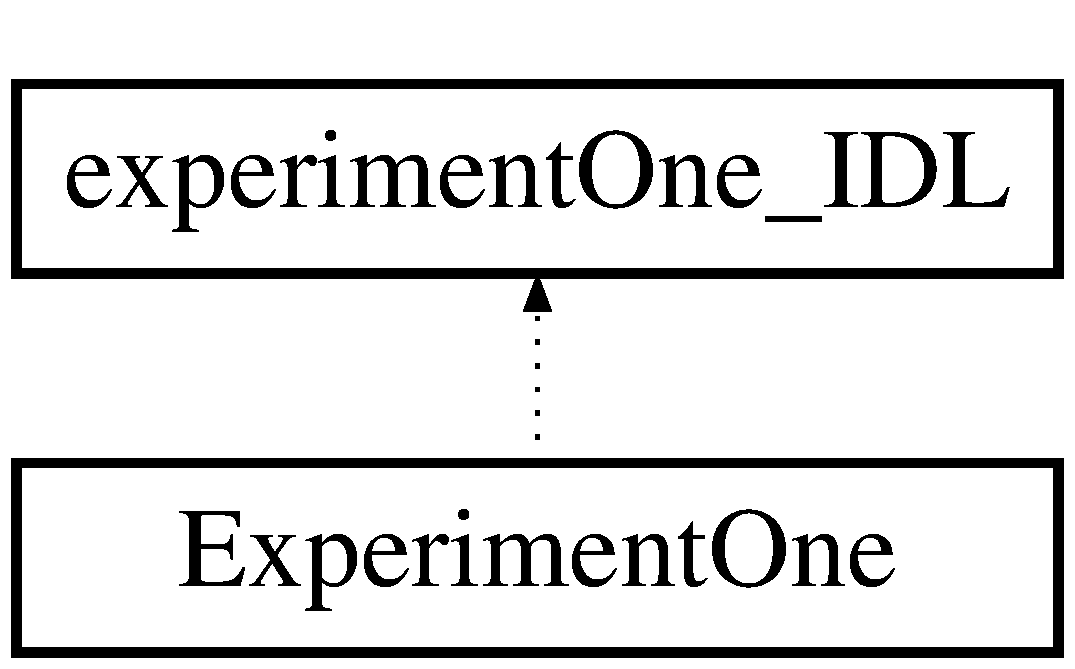
\includegraphics[height=2.000000cm]{classexperimentOne__IDL}
\end{center}
\end{figure}
\subsection*{Public Member Functions}
\begin{DoxyCompactItemize}
\item 
virtual yarp\-::os\-::\-Bottle \hyperlink{classexperimentOne__IDL_a4e631c4039aa9e4685f7d75f778145a2}{get\-\_\-blob} ()
\begin{DoxyCompactList}\small\item\em Send the current 2\-D blob. \end{DoxyCompactList}\item 
virtual bool \hyperlink{classexperimentOne__IDL_a3ba4eae42268c1dec8c90a971ffde7af}{set\-\_\-object\-\_\-name} (const std\-::string \&entry)
\begin{DoxyCompactList}\small\item\em Set the name of the object (stored by the object property collector). \end{DoxyCompactList}\item 
virtual std\-::string \hyperlink{classexperimentOne__IDL_af9d945019f95b6f806a20615e56b7c4b}{get\-\_\-object\-\_\-name} ()
\begin{DoxyCompactList}\small\item\em Get the name of the object. \end{DoxyCompactList}\item 
virtual bool \hyperlink{classexperimentOne__IDL_ab628b9a3d8ada84e07aaadf891a7ccd0}{go\-\_\-next} ()
\begin{DoxyCompactList}\small\item\em Ask to go to the next step, following the pipeline\-: 1-\/ compute superquadric 2-\/ compute pose 3-\/ ask the robot to move. \end{DoxyCompactList}\item 
virtual bool \hyperlink{classexperimentOne__IDL_a3d5c2f8f904ef29753934d10df4717a4}{start\-\_\-from\-\_\-scratch} ()
\begin{DoxyCompactList}\small\item\em The pipeline is restarted and is waiting the command \char`\"{}go\-\_\-next\char`\"{} to start from step 1. \end{DoxyCompactList}\item 
virtual bool \hyperlink{classexperimentOne__IDL_a30aa180a17e099d11a6c0588dc96eed1}{acquire\-\_\-superq} ()
\begin{DoxyCompactList}\small\item\em If you want just to perform step 1. \end{DoxyCompactList}\item 
virtual bool \hyperlink{classexperimentOne__IDL_a60389d324212814aa2dce49ed321e184}{compute\-\_\-pose} ()
\begin{DoxyCompactList}\small\item\em If you want just to perform step 2 (if step 1 has been performed). \end{DoxyCompactList}\item 
virtual bool \hyperlink{classexperimentOne__IDL_a2c72862f31d34a4e12adeb1e1289b5f0}{grasp\-\_\-object} ()
\begin{DoxyCompactList}\small\item\em If you want just to perform step 3 (if step 2 has been performed). \end{DoxyCompactList}\item 
virtual bool \hyperlink{classexperimentOne__IDL_a22c8d88117619d4e32ccc46efb455839}{go\-\_\-back\-\_\-home} ()
\begin{DoxyCompactList}\small\item\em Ask the robot to stop and go back to home position with the arm that is moving. \end{DoxyCompactList}\item 
virtual bool \hyperlink{classexperimentOne__IDL_a271373576b352956b3d7b2c111db3e40}{clear\-\_\-poses} ()
\begin{DoxyCompactList}\small\item\em Clear all the computed poses. \end{DoxyCompactList}\item 
virtual bool \hyperlink{classexperimentOne__IDL_acb2bfe937ed1900166744fce3a8f4cab}{set\-\_\-hand\-\_\-for\-\_\-computation} (const std\-::string \&entry)
\begin{DoxyCompactList}\small\item\em Set the hand for pose computation. \end{DoxyCompactList}\item 
virtual std\-::string \hyperlink{classexperimentOne__IDL_a93141c9f92c9c7a17518c3ddafda1fa4}{get\-\_\-hand\-\_\-for\-\_\-computation} ()
\begin{DoxyCompactList}\small\item\em Get the hand for pose computation. \end{DoxyCompactList}\item 
virtual bool \hyperlink{classexperimentOne__IDL_a0422e6ffaef0e60e1a557a342aeb5d4a}{set\-\_\-hand\-\_\-for\-\_\-moving} (const std\-::string \&entry)
\begin{DoxyCompactList}\small\item\em Set the hand for moving. \end{DoxyCompactList}\item 
virtual std\-::string \hyperlink{classexperimentOne__IDL_a9b24bdfe4b5bff2970a63126ca100706}{get\-\_\-hand\-\_\-for\-\_\-moving} ()
\begin{DoxyCompactList}\small\item\em Get the hand for pose computation. \end{DoxyCompactList}\item 
virtual std\-::string \hyperlink{classexperimentOne__IDL_a5cfa4d56fb13586ba889ff11031e88d1}{get\-\_\-automatic\-\_\-hand} ()
\begin{DoxyCompactList}\small\item\em Get if automatic selection of the hand is on or off. \end{DoxyCompactList}\item 
virtual bool \hyperlink{classexperimentOne__IDL_a1612f36ed85af9e6dbc595405e733977}{set\-\_\-automatic\-\_\-hand} (const std\-::string \&entry)
\begin{DoxyCompactList}\small\item\em Set if automatic selection of the hand is on or off. \end{DoxyCompactList}\item 
virtual bool \hyperlink{classexperimentOne__IDL_a36a7306993eeae5778bacac4f4154126}{set\-\_\-filtered\-\_\-superq} (const std\-::string \&entry)
\begin{DoxyCompactList}\small\item\em Set if to ask the filtered superquadric or not. \end{DoxyCompactList}\item 
virtual std\-::string \hyperlink{classexperimentOne__IDL_a855625d91d880d87206c643a831c3453}{get\-\_\-filtered\-\_\-superq} ()
\begin{DoxyCompactList}\small\item\em Get if to ask the filtered superquadric or not. \end{DoxyCompactList}\item 
virtual bool \hyperlink{classexperimentOne__IDL_a0e42d009f1d2bfbaae9906c4775dd922}{set\-\_\-reset\-\_\-filter} (const std\-::string \&entry)
\begin{DoxyCompactList}\small\item\em Set if to reset the filtered superquadric or not. \end{DoxyCompactList}\item 
virtual std\-::string \hyperlink{classexperimentOne__IDL_aefa9eabe3c0b14707eb2d8e24f3e0312}{get\-\_\-reset\-\_\-filter} ()
\begin{DoxyCompactList}\small\item\em Get if to reset the filtered superquadric or not. \end{DoxyCompactList}\item 
virtual bool \hyperlink{classexperimentOne__IDL_a12be87d589038ab4ee9bc1adb902ac53}{set\-\_\-object\-\_\-class} (const std\-::string \&entry)
\begin{DoxyCompactList}\small\item\em Set the current object class. \end{DoxyCompactList}\item 
virtual std\-::string \hyperlink{classexperimentOne__IDL_acecb65b51331f47d97fb4a3a6cf15b42}{get\-\_\-object\-\_\-class} ()
\begin{DoxyCompactList}\small\item\em Get the current object class. \end{DoxyCompactList}\item 
virtual bool {\bfseries read} (yarp\-::os\-::\-Connection\-Reader \&connection) Y\-A\-R\-P\-\_\-\-O\-V\-E\-R\-R\-I\-D\-E\label{classexperimentOne__IDL_a3e02eb2decd566b824035195358abe0d}

\item 
virtual std\-::vector$<$ std\-::string $>$ {\bfseries help} (const std\-::string \&function\-Name=\char`\"{}-\/-\/all\char`\"{})\label{classexperimentOne__IDL_a758e17bcfb1b243915cd696eccd1ce5b}

\end{DoxyCompactItemize}


\subsection{Detailed Description}
\hyperlink{classexperimentOne__IDL}{experiment\-One\-\_\-\-I\-D\-L} I\-D\-L Interface to \hyperlink{group__experiment-1}{experiment-\/1} services. 

Definition at line 18 of file experiment\-One\-\_\-\-I\-D\-L.\-h.



\subsection{Member Function Documentation}
\index{experiment\-One\-\_\-\-I\-D\-L@{experiment\-One\-\_\-\-I\-D\-L}!acquire\-\_\-superq@{acquire\-\_\-superq}}
\index{acquire\-\_\-superq@{acquire\-\_\-superq}!experimentOne_IDL@{experiment\-One\-\_\-\-I\-D\-L}}
\subsubsection[{acquire\-\_\-superq}]{\setlength{\rightskip}{0pt plus 5cm}virtual bool experiment\-One\-\_\-\-I\-D\-L\-::acquire\-\_\-superq (
\begin{DoxyParamCaption}
{}
\end{DoxyParamCaption}
)\hspace{0.3cm}{\ttfamily [virtual]}}\label{classexperimentOne__IDL_a30aa180a17e099d11a6c0588dc96eed1}


If you want just to perform step 1. 

\begin{DoxyReturn}{Returns}
true. 
\end{DoxyReturn}


Reimplemented in \hyperlink{classExperimentOne_a28e92b0a8df58c9dfc77ddae39c642b5}{Experiment\-One}.

\index{experiment\-One\-\_\-\-I\-D\-L@{experiment\-One\-\_\-\-I\-D\-L}!clear\-\_\-poses@{clear\-\_\-poses}}
\index{clear\-\_\-poses@{clear\-\_\-poses}!experimentOne_IDL@{experiment\-One\-\_\-\-I\-D\-L}}
\subsubsection[{clear\-\_\-poses}]{\setlength{\rightskip}{0pt plus 5cm}virtual bool experiment\-One\-\_\-\-I\-D\-L\-::clear\-\_\-poses (
\begin{DoxyParamCaption}
{}
\end{DoxyParamCaption}
)\hspace{0.3cm}{\ttfamily [virtual]}}\label{classexperimentOne__IDL_a271373576b352956b3d7b2c111db3e40}


Clear all the computed poses. 

\begin{DoxyReturn}{Returns}
true. 
\end{DoxyReturn}


Reimplemented in \hyperlink{classExperimentOne_a827996b603991113f08c928ccd7e7793}{Experiment\-One}.

\index{experiment\-One\-\_\-\-I\-D\-L@{experiment\-One\-\_\-\-I\-D\-L}!compute\-\_\-pose@{compute\-\_\-pose}}
\index{compute\-\_\-pose@{compute\-\_\-pose}!experimentOne_IDL@{experiment\-One\-\_\-\-I\-D\-L}}
\subsubsection[{compute\-\_\-pose}]{\setlength{\rightskip}{0pt plus 5cm}virtual bool experiment\-One\-\_\-\-I\-D\-L\-::compute\-\_\-pose (
\begin{DoxyParamCaption}
{}
\end{DoxyParamCaption}
)\hspace{0.3cm}{\ttfamily [virtual]}}\label{classexperimentOne__IDL_a60389d324212814aa2dce49ed321e184}


If you want just to perform step 2 (if step 1 has been performed). 

\begin{DoxyReturn}{Returns}
true/false on success/failure. 
\end{DoxyReturn}


Reimplemented in \hyperlink{classExperimentOne_a39a4ec1aa004bcdc7a2b3cfb3804e59f}{Experiment\-One}.

\index{experiment\-One\-\_\-\-I\-D\-L@{experiment\-One\-\_\-\-I\-D\-L}!get\-\_\-automatic\-\_\-hand@{get\-\_\-automatic\-\_\-hand}}
\index{get\-\_\-automatic\-\_\-hand@{get\-\_\-automatic\-\_\-hand}!experimentOne_IDL@{experiment\-One\-\_\-\-I\-D\-L}}
\subsubsection[{get\-\_\-automatic\-\_\-hand}]{\setlength{\rightskip}{0pt plus 5cm}virtual std\-::string experiment\-One\-\_\-\-I\-D\-L\-::get\-\_\-automatic\-\_\-hand (
\begin{DoxyParamCaption}
{}
\end{DoxyParamCaption}
)\hspace{0.3cm}{\ttfamily [virtual]}}\label{classexperimentOne__IDL_a5cfa4d56fb13586ba889ff11031e88d1}


Get if automatic selection of the hand is on or off. 

\begin{DoxyReturn}{Returns}
\char`\"{}on\char`\"{} or \char`\"{}off\char`\"{}. 
\end{DoxyReturn}


Reimplemented in \hyperlink{classExperimentOne_a25eb29db579ef1d960c35bd2bc71ec36}{Experiment\-One}.

\index{experiment\-One\-\_\-\-I\-D\-L@{experiment\-One\-\_\-\-I\-D\-L}!get\-\_\-blob@{get\-\_\-blob}}
\index{get\-\_\-blob@{get\-\_\-blob}!experimentOne_IDL@{experiment\-One\-\_\-\-I\-D\-L}}
\subsubsection[{get\-\_\-blob}]{\setlength{\rightskip}{0pt plus 5cm}virtual yarp\-::os\-::\-Bottle experiment\-One\-\_\-\-I\-D\-L\-::get\-\_\-blob (
\begin{DoxyParamCaption}
{}
\end{DoxyParamCaption}
)\hspace{0.3cm}{\ttfamily [virtual]}}\label{classexperimentOne__IDL_a4e631c4039aa9e4685f7d75f778145a2}


Send the current 2\-D blob. 

\begin{DoxyReturn}{Returns}
a bottle containing all the 2\-D points of the blob 
\end{DoxyReturn}
\index{experiment\-One\-\_\-\-I\-D\-L@{experiment\-One\-\_\-\-I\-D\-L}!get\-\_\-filtered\-\_\-superq@{get\-\_\-filtered\-\_\-superq}}
\index{get\-\_\-filtered\-\_\-superq@{get\-\_\-filtered\-\_\-superq}!experimentOne_IDL@{experiment\-One\-\_\-\-I\-D\-L}}
\subsubsection[{get\-\_\-filtered\-\_\-superq}]{\setlength{\rightskip}{0pt plus 5cm}virtual std\-::string experiment\-One\-\_\-\-I\-D\-L\-::get\-\_\-filtered\-\_\-superq (
\begin{DoxyParamCaption}
{}
\end{DoxyParamCaption}
)\hspace{0.3cm}{\ttfamily [virtual]}}\label{classexperimentOne__IDL_a855625d91d880d87206c643a831c3453}


Get if to ask the filtered superquadric or not. 

\begin{DoxyReturn}{Returns}
true/false on success/failure. 
\end{DoxyReturn}


Reimplemented in \hyperlink{classExperimentOne_a4fcbf7d582b26a64f67fc7d05f578e41}{Experiment\-One}.

\index{experiment\-One\-\_\-\-I\-D\-L@{experiment\-One\-\_\-\-I\-D\-L}!get\-\_\-hand\-\_\-for\-\_\-computation@{get\-\_\-hand\-\_\-for\-\_\-computation}}
\index{get\-\_\-hand\-\_\-for\-\_\-computation@{get\-\_\-hand\-\_\-for\-\_\-computation}!experimentOne_IDL@{experiment\-One\-\_\-\-I\-D\-L}}
\subsubsection[{get\-\_\-hand\-\_\-for\-\_\-computation}]{\setlength{\rightskip}{0pt plus 5cm}virtual std\-::string experiment\-One\-\_\-\-I\-D\-L\-::get\-\_\-hand\-\_\-for\-\_\-computation (
\begin{DoxyParamCaption}
{}
\end{DoxyParamCaption}
)\hspace{0.3cm}{\ttfamily [virtual]}}\label{classexperimentOne__IDL_a93141c9f92c9c7a17518c3ddafda1fa4}


Get the hand for pose computation. 

\begin{DoxyReturn}{Returns}
\char`\"{}right\char`\"{}, \char`\"{}left\char`\"{} or \char`\"{}both\char`\"{}. 
\end{DoxyReturn}


Reimplemented in \hyperlink{classExperimentOne_aef03af801993c3d869f0eedde21388dd}{Experiment\-One}.

\index{experiment\-One\-\_\-\-I\-D\-L@{experiment\-One\-\_\-\-I\-D\-L}!get\-\_\-hand\-\_\-for\-\_\-moving@{get\-\_\-hand\-\_\-for\-\_\-moving}}
\index{get\-\_\-hand\-\_\-for\-\_\-moving@{get\-\_\-hand\-\_\-for\-\_\-moving}!experimentOne_IDL@{experiment\-One\-\_\-\-I\-D\-L}}
\subsubsection[{get\-\_\-hand\-\_\-for\-\_\-moving}]{\setlength{\rightskip}{0pt plus 5cm}virtual std\-::string experiment\-One\-\_\-\-I\-D\-L\-::get\-\_\-hand\-\_\-for\-\_\-moving (
\begin{DoxyParamCaption}
{}
\end{DoxyParamCaption}
)\hspace{0.3cm}{\ttfamily [virtual]}}\label{classexperimentOne__IDL_a9b24bdfe4b5bff2970a63126ca100706}


Get the hand for pose computation. 

\begin{DoxyReturn}{Returns}
\char`\"{}right\char`\"{}, \char`\"{}left\char`\"{} or \char`\"{}both\char`\"{}. 
\end{DoxyReturn}


Reimplemented in \hyperlink{classExperimentOne_a066ac71cee6dec9422f213b2a58f21ba}{Experiment\-One}.

\index{experiment\-One\-\_\-\-I\-D\-L@{experiment\-One\-\_\-\-I\-D\-L}!get\-\_\-object\-\_\-class@{get\-\_\-object\-\_\-class}}
\index{get\-\_\-object\-\_\-class@{get\-\_\-object\-\_\-class}!experimentOne_IDL@{experiment\-One\-\_\-\-I\-D\-L}}
\subsubsection[{get\-\_\-object\-\_\-class}]{\setlength{\rightskip}{0pt plus 5cm}virtual std\-::string experiment\-One\-\_\-\-I\-D\-L\-::get\-\_\-object\-\_\-class (
\begin{DoxyParamCaption}
{}
\end{DoxyParamCaption}
)\hspace{0.3cm}{\ttfamily [virtual]}}\label{classexperimentOne__IDL_acecb65b51331f47d97fb4a3a6cf15b42}


Get the current object class. 

\begin{DoxyReturn}{Returns}
the current object class. 
\end{DoxyReturn}


Reimplemented in \hyperlink{classExperimentOne_a43cf934e2479fd6ef87be9048800a489}{Experiment\-One}.

\index{experiment\-One\-\_\-\-I\-D\-L@{experiment\-One\-\_\-\-I\-D\-L}!get\-\_\-object\-\_\-name@{get\-\_\-object\-\_\-name}}
\index{get\-\_\-object\-\_\-name@{get\-\_\-object\-\_\-name}!experimentOne_IDL@{experiment\-One\-\_\-\-I\-D\-L}}
\subsubsection[{get\-\_\-object\-\_\-name}]{\setlength{\rightskip}{0pt plus 5cm}virtual std\-::string experiment\-One\-\_\-\-I\-D\-L\-::get\-\_\-object\-\_\-name (
\begin{DoxyParamCaption}
{}
\end{DoxyParamCaption}
)\hspace{0.3cm}{\ttfamily [virtual]}}\label{classexperimentOne__IDL_af9d945019f95b6f806a20615e56b7c4b}


Get the name of the object. 

\begin{DoxyReturn}{Returns}
a string with the name of the object. 
\end{DoxyReturn}


Reimplemented in \hyperlink{classExperimentOne_ac087378ef3308b52cef17a2fc9d80dfe}{Experiment\-One}.

\index{experiment\-One\-\_\-\-I\-D\-L@{experiment\-One\-\_\-\-I\-D\-L}!get\-\_\-reset\-\_\-filter@{get\-\_\-reset\-\_\-filter}}
\index{get\-\_\-reset\-\_\-filter@{get\-\_\-reset\-\_\-filter}!experimentOne_IDL@{experiment\-One\-\_\-\-I\-D\-L}}
\subsubsection[{get\-\_\-reset\-\_\-filter}]{\setlength{\rightskip}{0pt plus 5cm}virtual std\-::string experiment\-One\-\_\-\-I\-D\-L\-::get\-\_\-reset\-\_\-filter (
\begin{DoxyParamCaption}
{}
\end{DoxyParamCaption}
)\hspace{0.3cm}{\ttfamily [virtual]}}\label{classexperimentOne__IDL_aefa9eabe3c0b14707eb2d8e24f3e0312}


Get if to reset the filtered superquadric or not. 

\begin{DoxyReturn}{Returns}
true/false on success/failure. 
\end{DoxyReturn}


Reimplemented in \hyperlink{classExperimentOne_a3573bd59ace3a48477beefb75d544326}{Experiment\-One}.

\index{experiment\-One\-\_\-\-I\-D\-L@{experiment\-One\-\_\-\-I\-D\-L}!go\-\_\-back\-\_\-home@{go\-\_\-back\-\_\-home}}
\index{go\-\_\-back\-\_\-home@{go\-\_\-back\-\_\-home}!experimentOne_IDL@{experiment\-One\-\_\-\-I\-D\-L}}
\subsubsection[{go\-\_\-back\-\_\-home}]{\setlength{\rightskip}{0pt plus 5cm}virtual bool experiment\-One\-\_\-\-I\-D\-L\-::go\-\_\-back\-\_\-home (
\begin{DoxyParamCaption}
{}
\end{DoxyParamCaption}
)\hspace{0.3cm}{\ttfamily [virtual]}}\label{classexperimentOne__IDL_a22c8d88117619d4e32ccc46efb455839}


Ask the robot to stop and go back to home position with the arm that is moving. 

\begin{DoxyReturn}{Returns}
true/false on success/failure. 
\end{DoxyReturn}


Reimplemented in \hyperlink{classExperimentOne_a967da7276e9bee19c45c8a000bf1cb01}{Experiment\-One}.

\index{experiment\-One\-\_\-\-I\-D\-L@{experiment\-One\-\_\-\-I\-D\-L}!go\-\_\-next@{go\-\_\-next}}
\index{go\-\_\-next@{go\-\_\-next}!experimentOne_IDL@{experiment\-One\-\_\-\-I\-D\-L}}
\subsubsection[{go\-\_\-next}]{\setlength{\rightskip}{0pt plus 5cm}virtual bool experiment\-One\-\_\-\-I\-D\-L\-::go\-\_\-next (
\begin{DoxyParamCaption}
{}
\end{DoxyParamCaption}
)\hspace{0.3cm}{\ttfamily [virtual]}}\label{classexperimentOne__IDL_ab628b9a3d8ada84e07aaadf891a7ccd0}


Ask to go to the next step, following the pipeline\-: 1-\/ compute superquadric 2-\/ compute pose 3-\/ ask the robot to move. 

\begin{DoxyReturn}{Returns}
true. 
\end{DoxyReturn}


Reimplemented in \hyperlink{classExperimentOne_a6ce79bc38d0e6fc201db5576a2c9e265}{Experiment\-One}.

\index{experiment\-One\-\_\-\-I\-D\-L@{experiment\-One\-\_\-\-I\-D\-L}!grasp\-\_\-object@{grasp\-\_\-object}}
\index{grasp\-\_\-object@{grasp\-\_\-object}!experimentOne_IDL@{experiment\-One\-\_\-\-I\-D\-L}}
\subsubsection[{grasp\-\_\-object}]{\setlength{\rightskip}{0pt plus 5cm}virtual bool experiment\-One\-\_\-\-I\-D\-L\-::grasp\-\_\-object (
\begin{DoxyParamCaption}
{}
\end{DoxyParamCaption}
)\hspace{0.3cm}{\ttfamily [virtual]}}\label{classexperimentOne__IDL_a2c72862f31d34a4e12adeb1e1289b5f0}


If you want just to perform step 3 (if step 2 has been performed). 

\begin{DoxyReturn}{Returns}
true/false on success/failure. 
\end{DoxyReturn}


Reimplemented in \hyperlink{classExperimentOne_a9a2ab97ed5ae9420e352a20b01feda90}{Experiment\-One}.

\index{experiment\-One\-\_\-\-I\-D\-L@{experiment\-One\-\_\-\-I\-D\-L}!set\-\_\-automatic\-\_\-hand@{set\-\_\-automatic\-\_\-hand}}
\index{set\-\_\-automatic\-\_\-hand@{set\-\_\-automatic\-\_\-hand}!experimentOne_IDL@{experiment\-One\-\_\-\-I\-D\-L}}
\subsubsection[{set\-\_\-automatic\-\_\-hand}]{\setlength{\rightskip}{0pt plus 5cm}virtual bool experiment\-One\-\_\-\-I\-D\-L\-::set\-\_\-automatic\-\_\-hand (
\begin{DoxyParamCaption}
\item[{const std\-::string \&}]{entry}
\end{DoxyParamCaption}
)\hspace{0.3cm}{\ttfamily [virtual]}}\label{classexperimentOne__IDL_a1612f36ed85af9e6dbc595405e733977}


Set if automatic selection of the hand is on or off. 


\begin{DoxyParams}{Parameters}
{\em entry} & can be \char`\"{}on\char`\"{} or \char`\"{}off\char`\"{} \\
\hline
\end{DoxyParams}
\begin{DoxyReturn}{Returns}
true/false on success/failure. 
\end{DoxyReturn}
\index{experiment\-One\-\_\-\-I\-D\-L@{experiment\-One\-\_\-\-I\-D\-L}!set\-\_\-filtered\-\_\-superq@{set\-\_\-filtered\-\_\-superq}}
\index{set\-\_\-filtered\-\_\-superq@{set\-\_\-filtered\-\_\-superq}!experimentOne_IDL@{experiment\-One\-\_\-\-I\-D\-L}}
\subsubsection[{set\-\_\-filtered\-\_\-superq}]{\setlength{\rightskip}{0pt plus 5cm}virtual bool experiment\-One\-\_\-\-I\-D\-L\-::set\-\_\-filtered\-\_\-superq (
\begin{DoxyParamCaption}
\item[{const std\-::string \&}]{entry}
\end{DoxyParamCaption}
)\hspace{0.3cm}{\ttfamily [virtual]}}\label{classexperimentOne__IDL_a36a7306993eeae5778bacac4f4154126}


Set if to ask the filtered superquadric or not. 


\begin{DoxyParams}{Parameters}
{\em entry} & can be \char`\"{}on\char`\"{} or \char`\"{}off\char`\"{}. \\
\hline
\end{DoxyParams}
\begin{DoxyReturn}{Returns}
\char`\"{}on\char`\"{} or \char`\"{}off\char`\"{}. 
\end{DoxyReturn}
\index{experiment\-One\-\_\-\-I\-D\-L@{experiment\-One\-\_\-\-I\-D\-L}!set\-\_\-hand\-\_\-for\-\_\-computation@{set\-\_\-hand\-\_\-for\-\_\-computation}}
\index{set\-\_\-hand\-\_\-for\-\_\-computation@{set\-\_\-hand\-\_\-for\-\_\-computation}!experimentOne_IDL@{experiment\-One\-\_\-\-I\-D\-L}}
\subsubsection[{set\-\_\-hand\-\_\-for\-\_\-computation}]{\setlength{\rightskip}{0pt plus 5cm}virtual bool experiment\-One\-\_\-\-I\-D\-L\-::set\-\_\-hand\-\_\-for\-\_\-computation (
\begin{DoxyParamCaption}
\item[{const std\-::string \&}]{entry}
\end{DoxyParamCaption}
)\hspace{0.3cm}{\ttfamily [virtual]}}\label{classexperimentOne__IDL_acb2bfe937ed1900166744fce3a8f4cab}


Set the hand for pose computation. 


\begin{DoxyParams}{Parameters}
{\em entry} & can be \char`\"{}right\char`\"{}, \char`\"{}left\char`\"{} or \char`\"{}both\char`\"{}. \\
\hline
\end{DoxyParams}
\begin{DoxyReturn}{Returns}
true/false on success/failure. 
\end{DoxyReturn}
\index{experiment\-One\-\_\-\-I\-D\-L@{experiment\-One\-\_\-\-I\-D\-L}!set\-\_\-hand\-\_\-for\-\_\-moving@{set\-\_\-hand\-\_\-for\-\_\-moving}}
\index{set\-\_\-hand\-\_\-for\-\_\-moving@{set\-\_\-hand\-\_\-for\-\_\-moving}!experimentOne_IDL@{experiment\-One\-\_\-\-I\-D\-L}}
\subsubsection[{set\-\_\-hand\-\_\-for\-\_\-moving}]{\setlength{\rightskip}{0pt plus 5cm}virtual bool experiment\-One\-\_\-\-I\-D\-L\-::set\-\_\-hand\-\_\-for\-\_\-moving (
\begin{DoxyParamCaption}
\item[{const std\-::string \&}]{entry}
\end{DoxyParamCaption}
)\hspace{0.3cm}{\ttfamily [virtual]}}\label{classexperimentOne__IDL_a0422e6ffaef0e60e1a557a342aeb5d4a}


Set the hand for moving. 


\begin{DoxyParams}{Parameters}
{\em entry} & can be \char`\"{}right\char`\"{} or \char`\"{}left\char`\"{}. \\
\hline
\end{DoxyParams}
\begin{DoxyReturn}{Returns}
true/false on success/failure. 
\end{DoxyReturn}
\index{experiment\-One\-\_\-\-I\-D\-L@{experiment\-One\-\_\-\-I\-D\-L}!set\-\_\-object\-\_\-class@{set\-\_\-object\-\_\-class}}
\index{set\-\_\-object\-\_\-class@{set\-\_\-object\-\_\-class}!experimentOne_IDL@{experiment\-One\-\_\-\-I\-D\-L}}
\subsubsection[{set\-\_\-object\-\_\-class}]{\setlength{\rightskip}{0pt plus 5cm}virtual bool experiment\-One\-\_\-\-I\-D\-L\-::set\-\_\-object\-\_\-class (
\begin{DoxyParamCaption}
\item[{const std\-::string \&}]{entry}
\end{DoxyParamCaption}
)\hspace{0.3cm}{\ttfamily [virtual]}}\label{classexperimentOne__IDL_a12be87d589038ab4ee9bc1adb902ac53}


Set the current object class. 


\begin{DoxyParams}{Parameters}
{\em entry} & the name of the object class \\
\hline
\end{DoxyParams}
\begin{DoxyReturn}{Returns}
true/false on success/failure. 
\end{DoxyReturn}
\index{experiment\-One\-\_\-\-I\-D\-L@{experiment\-One\-\_\-\-I\-D\-L}!set\-\_\-object\-\_\-name@{set\-\_\-object\-\_\-name}}
\index{set\-\_\-object\-\_\-name@{set\-\_\-object\-\_\-name}!experimentOne_IDL@{experiment\-One\-\_\-\-I\-D\-L}}
\subsubsection[{set\-\_\-object\-\_\-name}]{\setlength{\rightskip}{0pt plus 5cm}virtual bool experiment\-One\-\_\-\-I\-D\-L\-::set\-\_\-object\-\_\-name (
\begin{DoxyParamCaption}
\item[{const std\-::string \&}]{entry}
\end{DoxyParamCaption}
)\hspace{0.3cm}{\ttfamily [virtual]}}\label{classexperimentOne__IDL_a3ba4eae42268c1dec8c90a971ffde7af}


Set the name of the object (stored by the object property collector). 


\begin{DoxyParams}{Parameters}
{\em entry} & is the name of the object \\
\hline
\end{DoxyParams}
\begin{DoxyReturn}{Returns}
true/false on success/failure. 
\end{DoxyReturn}
\index{experiment\-One\-\_\-\-I\-D\-L@{experiment\-One\-\_\-\-I\-D\-L}!set\-\_\-reset\-\_\-filter@{set\-\_\-reset\-\_\-filter}}
\index{set\-\_\-reset\-\_\-filter@{set\-\_\-reset\-\_\-filter}!experimentOne_IDL@{experiment\-One\-\_\-\-I\-D\-L}}
\subsubsection[{set\-\_\-reset\-\_\-filter}]{\setlength{\rightskip}{0pt plus 5cm}virtual bool experiment\-One\-\_\-\-I\-D\-L\-::set\-\_\-reset\-\_\-filter (
\begin{DoxyParamCaption}
\item[{const std\-::string \&}]{entry}
\end{DoxyParamCaption}
)\hspace{0.3cm}{\ttfamily [virtual]}}\label{classexperimentOne__IDL_a0e42d009f1d2bfbaae9906c4775dd922}


Set if to reset the filtered superquadric or not. 


\begin{DoxyParams}{Parameters}
{\em entry} & can be \char`\"{}on\char`\"{} or \char`\"{}off\char`\"{}. \\
\hline
\end{DoxyParams}
\begin{DoxyReturn}{Returns}
\char`\"{}on\char`\"{} or \char`\"{}off\char`\"{}. 
\end{DoxyReturn}
\index{experiment\-One\-\_\-\-I\-D\-L@{experiment\-One\-\_\-\-I\-D\-L}!start\-\_\-from\-\_\-scratch@{start\-\_\-from\-\_\-scratch}}
\index{start\-\_\-from\-\_\-scratch@{start\-\_\-from\-\_\-scratch}!experimentOne_IDL@{experiment\-One\-\_\-\-I\-D\-L}}
\subsubsection[{start\-\_\-from\-\_\-scratch}]{\setlength{\rightskip}{0pt plus 5cm}virtual bool experiment\-One\-\_\-\-I\-D\-L\-::start\-\_\-from\-\_\-scratch (
\begin{DoxyParamCaption}
{}
\end{DoxyParamCaption}
)\hspace{0.3cm}{\ttfamily [virtual]}}\label{classexperimentOne__IDL_a3d5c2f8f904ef29753934d10df4717a4}


The pipeline is restarted and is waiting the command \char`\"{}go\-\_\-next\char`\"{} to start from step 1. 

\begin{DoxyReturn}{Returns}
true. 
\end{DoxyReturn}


Reimplemented in \hyperlink{classExperimentOne_ac01beb32e67fd6067c273ae505060139}{Experiment\-One}.



The documentation for this class was generated from the following file\-:\begin{DoxyCompactItemize}
\item 
/home/gvezzani/\-Desktop/\-Ph\-D/\-Anno\-\_\-2/experiment-\/new-\/grasp/experiment-\/1/idl\-\_\-dox/experiment\-One\-\_\-\-I\-D\-L.\-h\end{DoxyCompactItemize}

%--- End generated contents ---

% Index
\newpage
\phantomsection
\addcontentsline{toc}{chapter}{Index}
\printindex

\end{document}
